\documentclass{article}
\usepackage{geometry}                % See geometry.pdf to learn the layout options. There are lots.
%\geometry{letterpaper}                   % ... or a4paper or a5paper or ...
%\geometry{landscape}                % Activate for for rotated page geometry
%\usepackage[parfill]{parIEEEabrvskip}    % Activate to begin paragraphs with an empty line rather than an indent
\usepackage{graphicx}
\usepackage{caption}
\usepackage{subcaption}
\usepackage{amssymb}
\usepackage{amsmath}
\usepackage{epstopdf}
\usepackage{amsthm}

\usepackage{pifont} % check and x marks
\newcommand{\cmark}{\ding{51}}
\newcommand{\xmark}{\ding{55}}

\newcommand{\gcc}{{\tt 403.gcc}~}
\newcommand{\svd}{{\tt dgesdd}~}
\newcommand{\svdone}{{\tt dgesdd}$_1$~}
\newcommand{\svdtwo}{{\tt dgesdd$_2$}~}
\newcommand{\svdthree}{{\tt dgesdd$_3$}~}
\newcommand{\svdfour}{{\tt dgesdd$_4$}~}
\newcommand{\svdfive}{{\tt dgesdd$_5$}~}
\newcommand{\svdsix}{{\tt dgesdd$_6$}~}


\newcommand{\row}{{\tt row\_major}~}
\newcommand{\col}{{\tt col\_major}~}

\usepackage{authblk}
\DeclareGraphicsRule{.tif}{png}{.png}{`convert #1 `dirname #1`/`basename #1 .tif`.png}

\newtheorem*{mydef}{Definition}
\title{Determinism, Complexity, and Predictability in Computer Performance\\
Quantifying structured complexity and its role in predictability: With applications to predicting computer performance.
\\ Quantifying Predictability through Structural Complexity
\\ Quantifying Predictability using Structural Complexity
}



\author[1]{Joshua Garland \thanks{joshua.garland@colorado.edu}}
\author[1]{Ryan James \thanks{ryan.james@colorado.edu}}
\author[1,2]{Elizabeth Bradley \thanks{lizb@colorado.edu}}
\affil[1]{Department of Computer Science\\
  University of Colorado at Boulder\\
  Colorado, USA
}
\affil[2]{Santa Fe Institute\\
  New Mexico, USA
}


%Version 1
%\author{
%  \IEEEauthorblockN{Joshua Garland}
%  \IEEEauthorblockA{Dept. of Computer Science\\
%    University of Colorado at Boulder\\
%    Colorado, USA\\
%    Email: joshua.garland@colorado.edu}
%  \and
%  \IEEEauthorblockN{Ryan G.~James}
%  \IEEEauthorblockA{Complexity Sciences Center \& Dept. of Physics\\
%    University of California at Davis\\
%    California, USA\\
%    Email: rgjames@ucdavis.edu}
%    \and
%      \IEEEauthorblockN{Elizabeth Bradley}
%         \IEEEauthorblockA{Santa Fe Institute \\
%    New Mexico, USA\\
%    }
%  \IEEEauthorblockA{Dept. of Computer Science\\
%    University of Colorado at Boulder\\
%    Colorado, USA\\
%    Email: lizb@colorado.edu}
%  }



 %\author{
 %  \IEEEauthorblockN{
 %    Joshua Garland\IEEEauthorrefmark{1},
 %    Ryan G.~James\IEEEauthorrefmark{1} and
 %    Elizabeth Bradley\IEEEauthorrefmark{1}\IEEEauthorrefmark{2}}
 %  \IEEEauthorblockA{
 %    \IEEEauthorrefmark{1}Dept. of Computer Science
 %    University of Colorado, Boulder, Colorado 80309-0430 USA\\
 %    Email: joshua.garland@colorado.edu, ryan.james@colorado.edu}
 %  \IEEEauthorblockA{
 %    \IEEEauthorrefmark{2}Santa Fe Institute, 1399 Hyde Park Road, Santa Fe, New Mexico 87501  USA\\
 %    Email: lizb@colorado.edu}
 %  % \IEEEauthorblockA{
 %  %   \IEEEauthorrefmark{3}Complexity Sciences Center \& Physics Dept., University of California, Davis, %California 95616 USA\\
%   %   Email: rgjames@ucdavis.edu}
% }

\begin{document}



\maketitle





\begin{abstract}
  Computers are deterministic dynamical systems \cite{mytkowicz09}.
  Among other things, that implies that one should be able to use
  deterministic forecast rules to predict aspects of their behavior.
  That statement is sometimes---but not always---true. The memory and
  processor loads of some simple programs are easy to predict, for
  example, but those of more-complex programs like {\tt gcc} are not.
%%%%%%%%%%%%%%%%%%%%%%
%% I had to change all the \verb|blah| entries because they caused
%% latex to barf if they were in figure captions.  Odd bug.
%%%%%%%%%%%%%%%%%%%%%%
  The goal of this paper is to determine why that is the case. We
  conjecture that, in practice, complexity can effectively overwhelm
  the predictive power of deterministic forecast models. To explore
  that, we build models of a number of performance traces from
  different programs running on different Intel-based computers. We
  then calculate the \emph{permutation entropy}---a temporal entropy
  metric that uses ordinal analysis---of those traces and correlate
  those values against the prediction success.
\end{abstract}

\section{Introduction}\label{sec:intro}
%\begin{it}
%Paragraph on computer performance, including citations to Todd paper
%and summary of the results that indicate that they're deterministic
%nonlinear dynamical systems.  Given that, we should be able to
%predict.  What benefits would accrue if we could do so: power mgmt,
%end world hunger [[this is my primary goal everyday :)]], etc.
%\end{it}
Things to add to introduction
\begin{enumerate}
\item Different kinds of complexity exist in time series and this makes choosing prediction models difficult 
\subitem NOTE: RW and chaos are both complex. One is predictable and one is not.

\item Make an argument that Computer Performance is a great testing ground as it omits signals that completely cover the spectrum of complexity \col \dots \gcc

\item When deterministic structure even complex structure exists that structure can be utilized for prediction. 
\item For noisy real-valued time series distinguishing randomness (WN,RW) complexity from structured nonlinear / chaotic /high period / high dimensional etc complexity is (until now) very hard. 
\subitem for this provide predictions of \gcc and \col side by side and discuss "How can we tell if we did a bad job because the method is inadequate vs the signal being too complex. Lead this into is it possible to tell if there exists structure in a time series to know if we should find a better model or not. Maybe even having 4 predictions. top being ARIMA of the above signals and bottom being LMA of the above signals. Show that one improved and one did not. Is it that we used the wrong method to predict or is it that we simply can't predict the signal better than a random walk due to high levels of internal signal complexity.



\item Introduce the two main contributions of the paper which are outlined at the begining of the results section

\end{enumerate}



Computers are among the most complex engineered artifacts in current
use.  Modern microprocessor chips contain multiple processing units
and multi-layer memories, for instance, and they use complicated
hardware/software strategies to move data and threads of computation
across those resources.  These features---along with all the others
that go into the design of these chips---make the patterns of their
processor loads and memory accesses highly complex and hard to
predict.  Accurate forecasts of these quantities, if one could
construct them, could be used to improve computer design.  If one
could predict that a particular computational thread would be bogged
down for the next 0.6 seconds waiting for data from main memory, for
instance, one could save power by putting that thread on hold for that
time period (e.g., by migrating it to a processing unit whose clock
speed is scaled back).  Computer performance traces are, however, very
complex.  Even a simple ``microkernel,'' like a three-line loop that
repeatedly initializes a matrix in column-major order, can produce
{\sl chaotic} performance traces \cite{mytkowicz09}, as shown in
Figure~\ref{fig:col-ts}, and chaos places fundamental limits on
predictability.
%
 \begin{figure}[htbp]
    \centering
    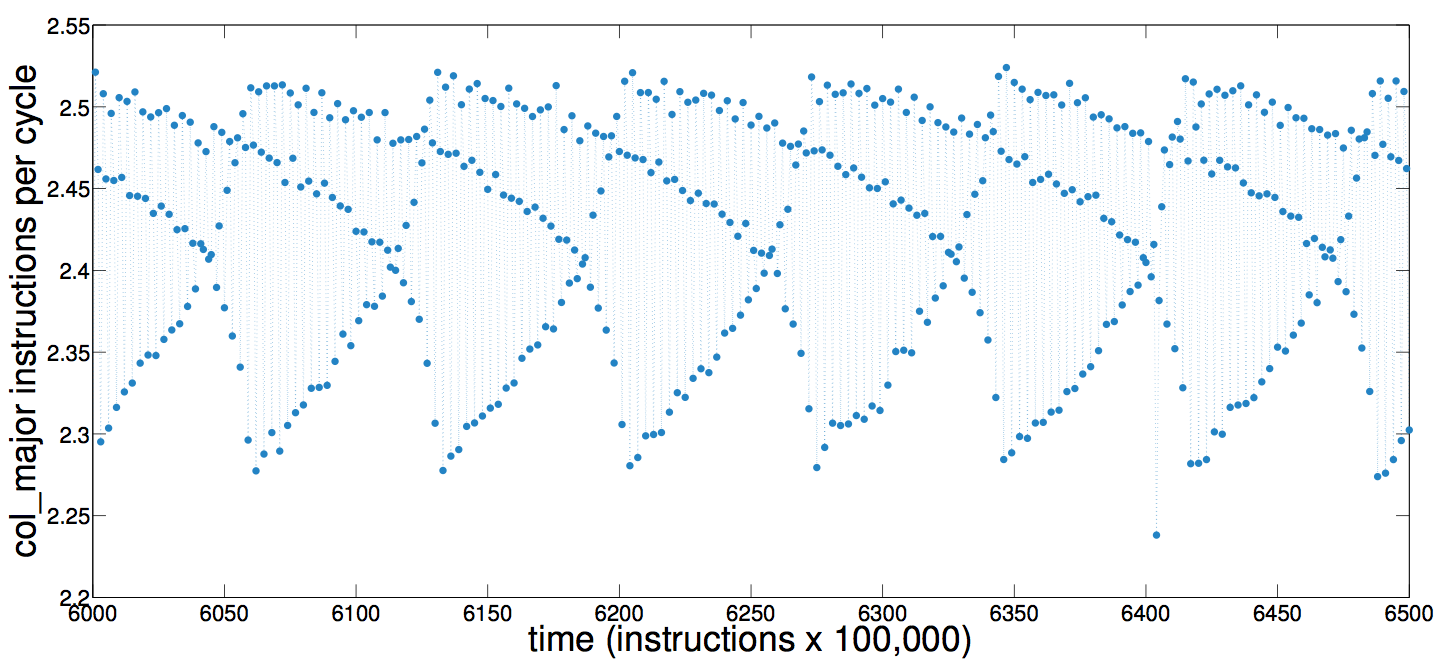
\includegraphics[width=\textwidth]{figs/colshortts}
    % where an .eps filename suffix will be assumed under latex,
    % and a .pdf suffix will be assumed for pdflatex
    \caption{A small snippet of the instructions per cycle(ipc) of {\tt
        \col}, a three-line C program that repeatedly initializes
      a matrix in column-major order, running on an Intel i7\textsuperscript{\textregistered}-based machine.  Even this
      simple program exhibits chaotic performance dynamics.}
   \label{fig:ipc}
  \end{figure}

\begin{figure}[htbp]
  \centering
  \begin{subfigure}[t]{0.475\textwidth}
    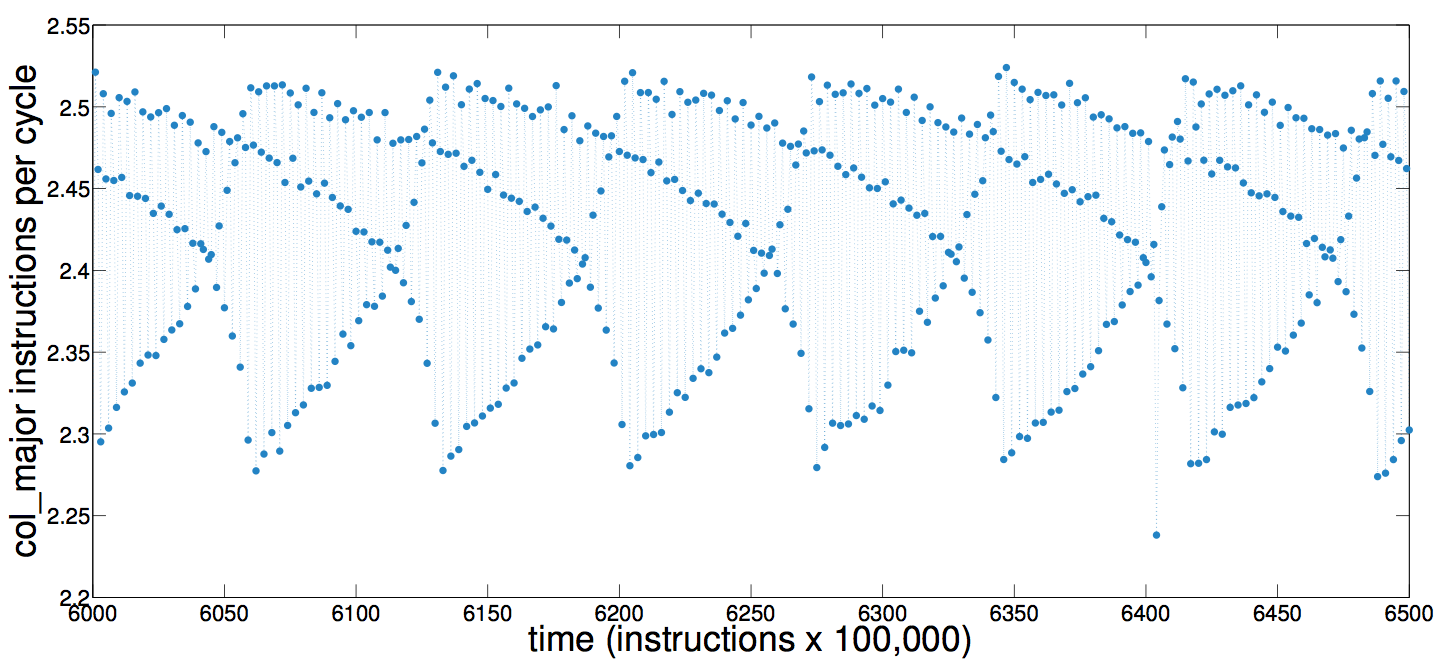
\includegraphics[width=0.95\textwidth]{figs/colshortts}
    \caption{A short segment of the instructions executed per CPU clock cycle
    (IPC) during the execution of \col. Each point is the IPC during a 100,000
    cycle period. There is a great deal of periodicity in this time series.}
    \label{fig:col-ts}
  \end{subfigure}%
  \begin{subfigure}[t]{0.475\textwidth}
    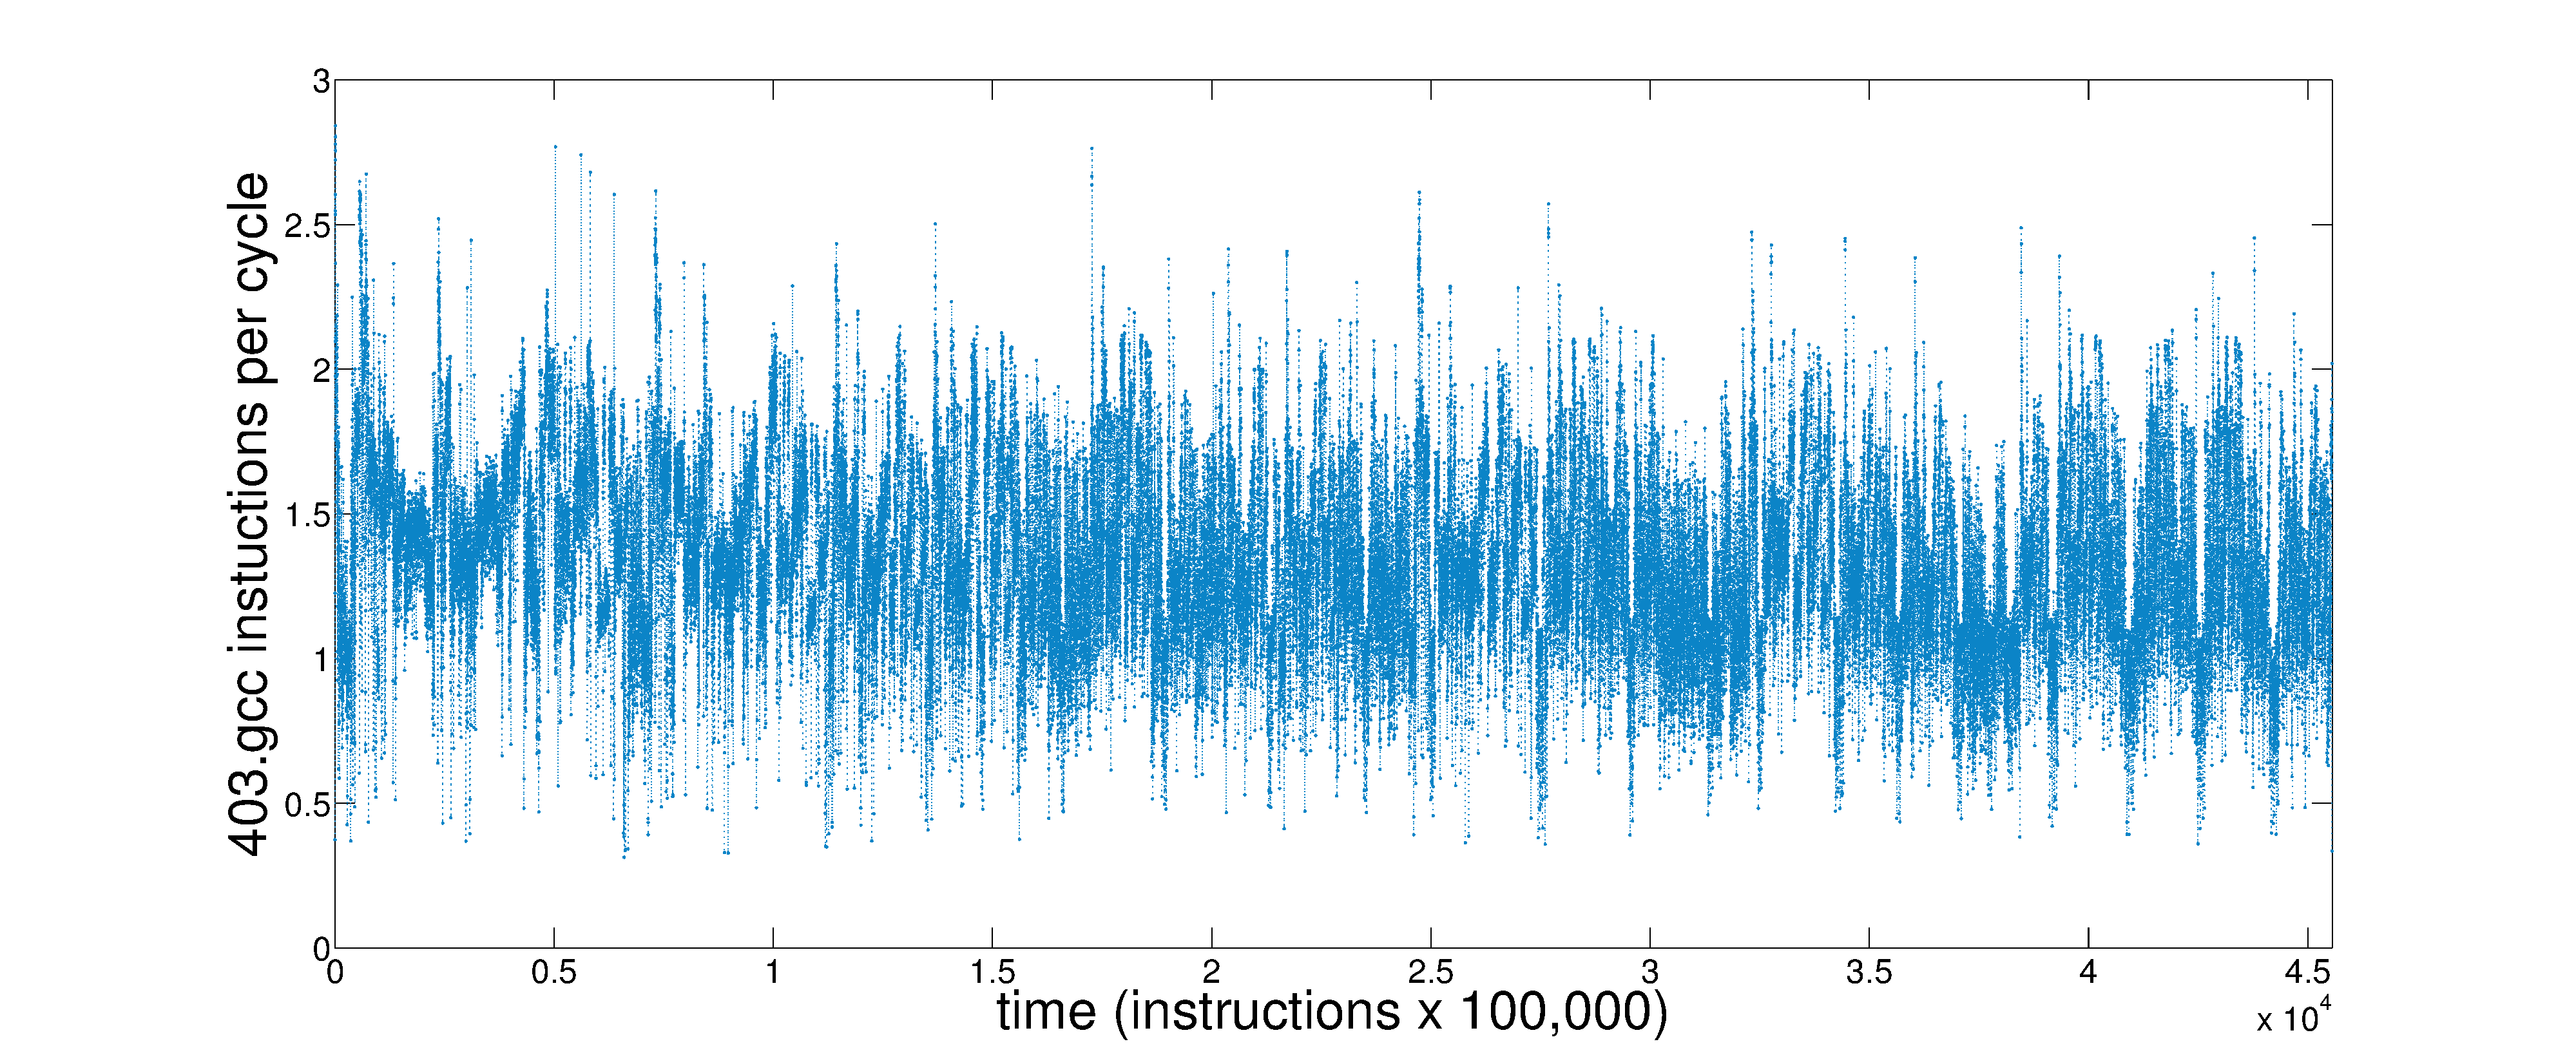
\includegraphics[width=0.95\textwidth]{figs/gccfullts}
    \caption{The full IPC time series during the execution of \gcc. This time
    series has very little structure.}
    \label{fig:gcc-ts}
  \end{subfigure}
  \label{fig:sample-ts}
\end{figure}




\begin{figure}[htbp]
  \centering
       
  \begin{subfigure}{0.5\textwidth}
    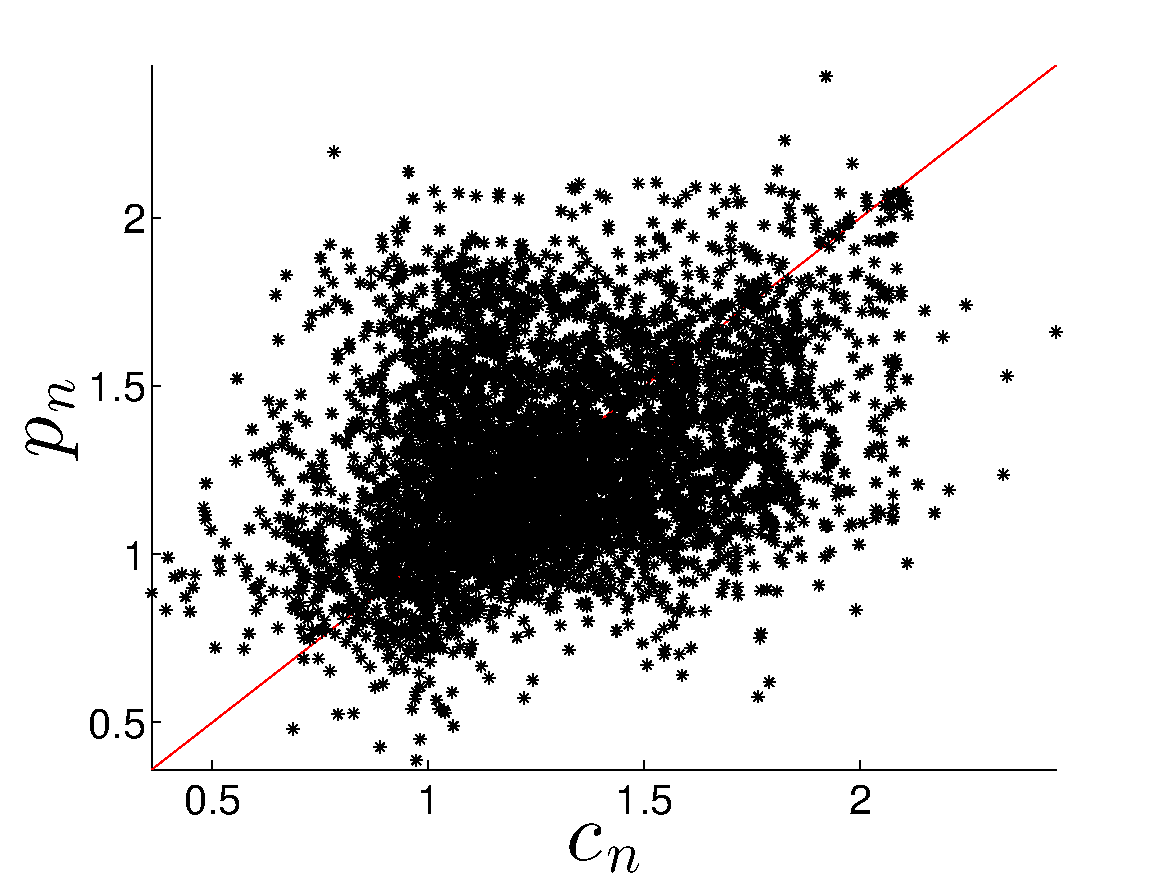
\includegraphics[width=\textwidth]{figs/gccARIMAForecast}
    \caption{\gcc ARIMA }
    \label{fig:gccARIMA}
  \end{subfigure}%
    \begin{subfigure}{0.5\textwidth}
    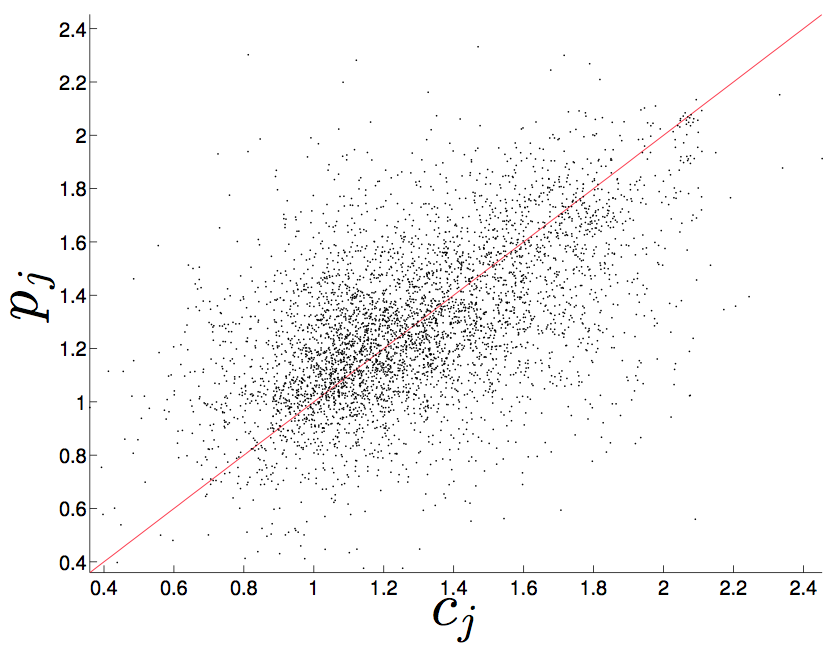
\includegraphics[width=\textwidth]{figs/gccLMAForecast}
    \caption{\gcc LMA}
    \label{fig:gccLMA}
  \end{subfigure}
  \\
  \begin{subfigure}{0.49\textwidth}
    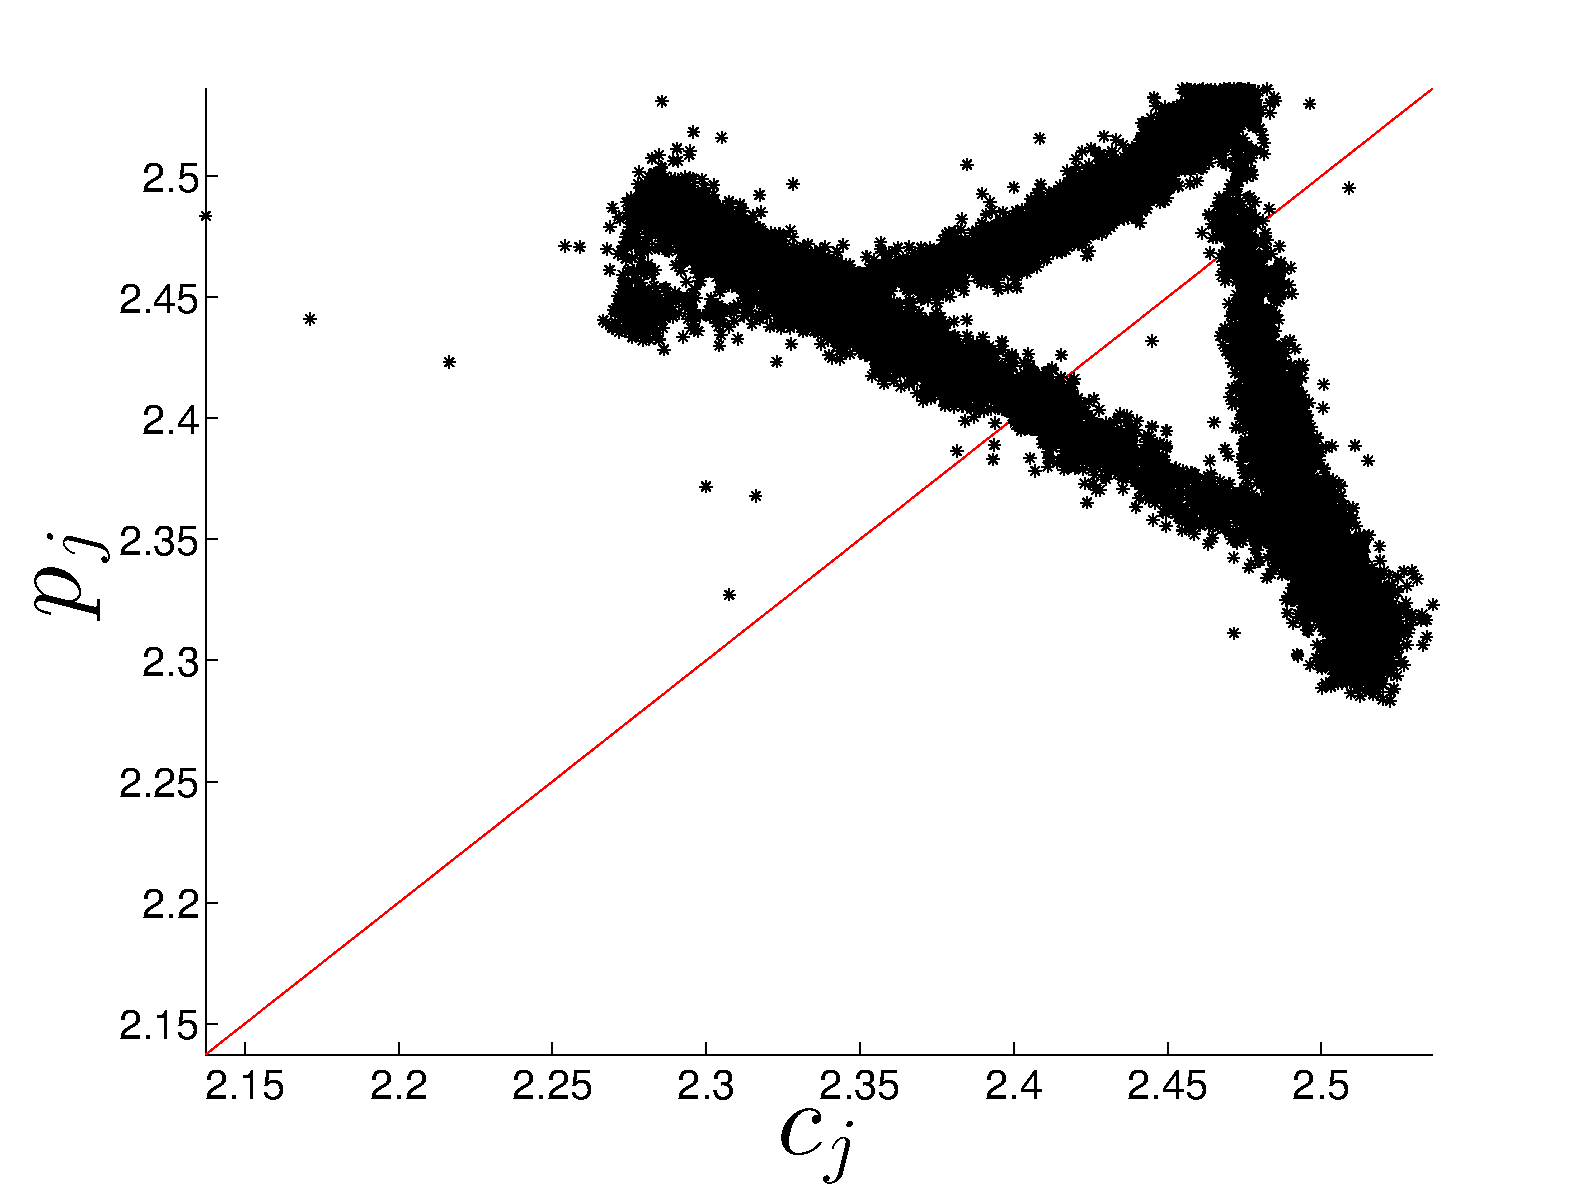
\includegraphics[width=\textwidth]{figs/colARIMAForecast}
    \caption{\col ARIMA}
    \label{fig:colARIMA}
  \end{subfigure}
    \begin{subfigure}{0.49\textwidth}
    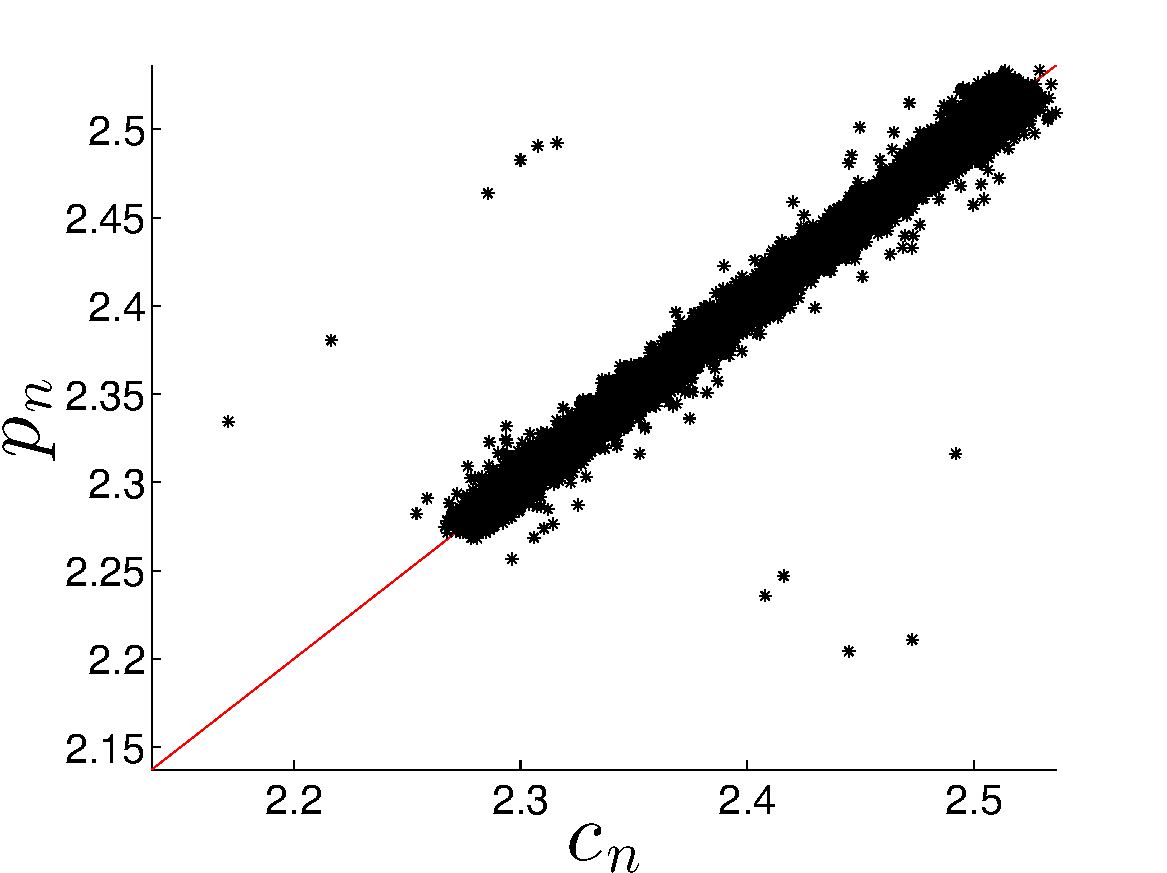
\includegraphics[width=\textwidth]{figs/colLMAForecast}
    \caption{\col LMA}
    \label{fig:colLMA}
  \end{subfigure}
  %\begin{subfigure}{0.5\textwidth}
  %  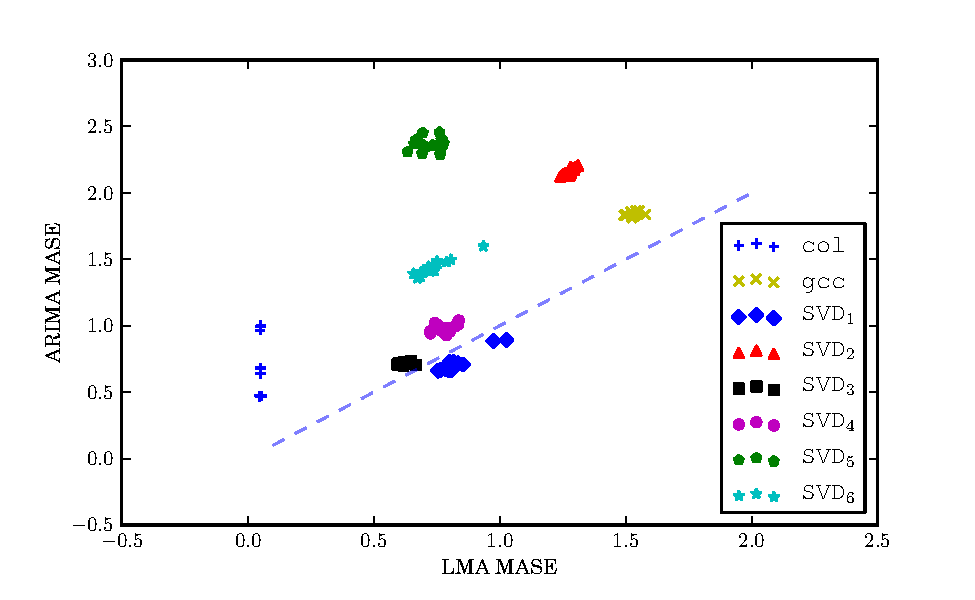
\includegraphics[width=1.0\textwidth]{figs/LMA_vs_ARIMA}
   \caption{
For each of these, we plot the predicted value $p_n$ against the correct value $c_n$. On this type of plot a perfect prediction lies exactly on the diagonal, that is the line $p_n = c_n$, e.g., \ref{fig:colLMA} is a near perfect prediction where-as \ref{fig:gccARIMA} is a very poor prediction. }\label{fig:gcc_vs_col}  
  %\end{subfigure}
\end{figure} 




The computer systems community has applied a variety of prediction
strategies to traces like this, most of which employ regression.  An
appealing alternative builds on the recently established fact that
computers can be effectively modeled as deterministic nonlinear
dynamical systems \cite{mytkowicz09}.  This result implies the
existence of a deterministic forecast rule for those dynamics.  In
particular, one can use \emph{delay-coordinate embedding} to
reconstruct the underlying dynamics of computer performance, then use
the resulting model to forecast the future values of computer
performance metrics such as memory or processor loads
\cite{josh-ida2011}.  In the case of simple microkernels like the one
that produced the trace in Figure~\ref{fig:ipc}, this deterministic
modeling and forecast strategy works very well.  In more-complicated
programs, however, such as speech recognition software or compilers,
this forecast strategy---as well as the traditional methods---break
down quickly.

This paper is a first step in understanding when, why, and how
deterministic forecast strategies fail when they are applied to
deterministic systems.  We focus here on the specific example of
computer performance.  We conjecture that the complexity of traces
from these systems---which results from the inherent dimension,
non-linearity, and non-stationarity of the dynamics, as well as from
measurement issues like noise, aggregation, and finite data
length---can make those deterministic signals \emph{effectively}
unpredictable.  We argue that \emph{permutation entropy}
\cite{bandt2002per}, a method for measuring the entropy of a
real-valued-finite-length time series through ordinal analysis, is an
effective way to explore that conjecture.  We study four
examples---two simple microkernels and two complex programs from the
SPEC benchmark suite---running on different Intel-based machines.  For
each program, we calculate the permutation entropy of the processor
load (instructions per cycle) and memory-use efficiency (cache-miss
rates), then compare that to the prediction accuracy attainable for
that trace using a simple deterministic model.

% paragraph to appease the theoretician in me
It is worth taking a moment to consider the theoretical possibility of
this task. We are not attempting to predict the state of the CPU at an
arbitrary point in the future --- this, at least with perfect
accuracy, would be tantamount to solving the halting problem. What we
are attempting is to predict aspects or functions of the running of
the CPU: instructions executed per second, cache misses per 100,000
instructions, and similar statistics. Prediction of these quantities
at some finite time in the future, even with perfect accuracy, does
not violate the Rice-Shapiro theorem.

% The rest of the paper is organized as follows.
% Section~\ref{sec:compModel} describes the experimental setup, as well
% as the nonlinear modeling and forecast strategies.  In
% Section~\ref{sec:meaComplex}, we review permutation entropy, calculate
% its value for a number of different computer performance traces, and
% compare the results to the prediction accuracy.  In
% Section~\ref{sec:conc}, we discuss these results and their
% implications in regard to our conjecture, and consider future areas of
% research.




\section{Experimental Methods and Modelling}\label{sec:compModel}

Section outline:

\begin{enumerate}
\item Experimental methods (how we collect the time series and what the times series are
\item Description of DCE and parameter estimation  
\item Description of auto ARIMA 
\subitem (this should be limited and explain it is meant to be out of the box) point at the paper for auto arima for more details.
\item Description of the two naive methods (random walk and mean), make sure to explain that these methods are naive and simple but not necessarily bad.
\item Add a section talking about evaluation methods i.e., MASE, this text is currently written and just sitting at the beginning of the results. 

\end{enumerate}



% took out for space
 \subsection{Reconstructing hidden dynamics}

Delay-coordinate embedding allows one to reconstruct a system's full
state-space dynamics from a \emph{single} scalar time-series
measurement---provided that some conditions hold regarding that data.
Specifically, if the underlying dynamics and the measurement
function---the mapping from the unknown state vector $\vec{X}$ to the
scalar value $x$ that one is measuring---are both smooth and generic,
Takens~\cite{takens} formally proves that the delay-coordinate map
\[
F(\tau,m)(x) = ([x(t) ~ x(t+\tau) ~ \dots ~x(t+m\tau)])
\]
from a $d$-dimensional smooth compact manifold $M$ to ${Re}^{2d+1}$,
where $t$ is time, is a diffeomorphism on $M$---in other words, that
the reconstructed dynamics and the true (hidden) dynamics have the
same topology.

This is an extremely powerful result: among other things, it means
that one can build a formal model of the full system dynamics without
measuring (or even knowing) every one of its state variables.  This is
the foundation of the modeling approach that is used in this paper.
The first step in the process is to estimate values for the two free
parameters in the delay-coordinate map: the delay $\tau$ and the
dimension $m$.  We follow standard procedures for this, choosing the
first minimum in the average mutual information as an estimate of
$\tau$ \cite{fraser-swinney} and using the false-near(est) neighbor
method of \cite{KBA92}, with a threshold of 10\%, to estimate $m$.  A
plot of the data from Figure~\ref{fig:ipc}, embedded following this
procedure, is shown in Figure~\ref{fig:embedding}.


 \begin{figure}
   \centering
     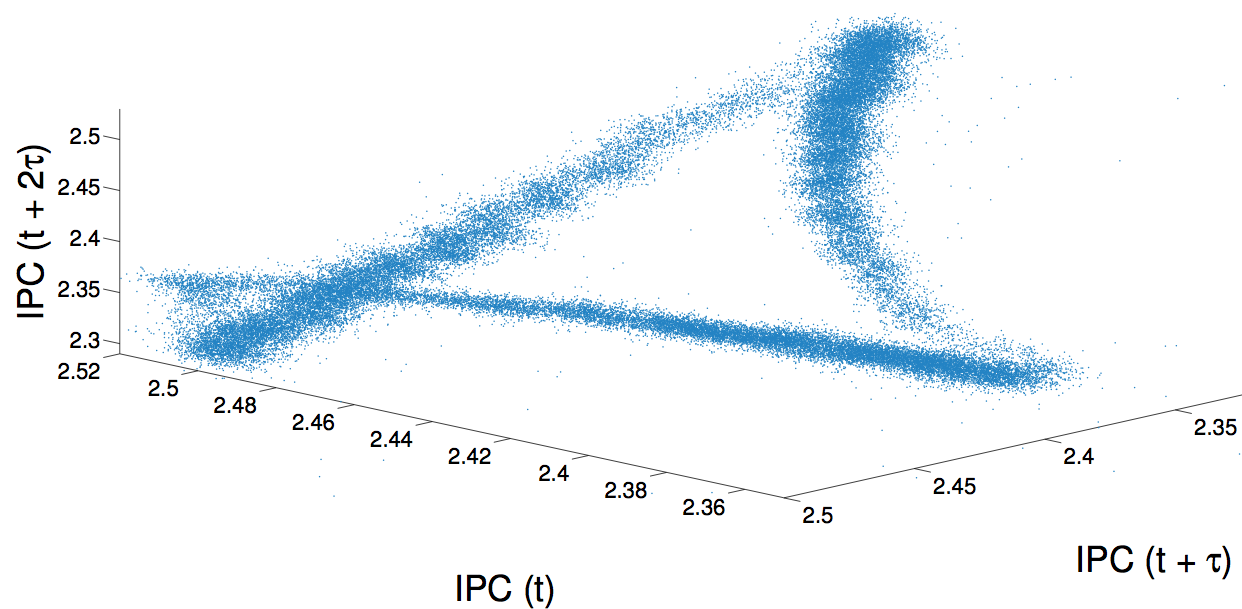
\includegraphics[width=\textwidth]{figs/colipc3d.png}
     \caption{A 3D projection of a delay-coordinate embedding of the trace
 from Figure~\ref{fig:ipc} with a delay ($\tau$) of 100,000 instructions.
 }
 \label{fig:embedding}
 \end{figure}


%% can cut for space if need be:
The coordinates of each point on this plot are differently delayed
elements of the \verb|col_major| L2 cache miss rate time series
$y(t)$: that is, $y(t)$ on the first axis, $y(t+\tau)$ on the second,
$y(t+2\tau)$ on the third, and so on.
%% ...down to here.
Structure in these kinds of plots---clearly visible in
Figure~\ref{fig:embedding}---is an indication of
determinism\footnote{A deeper analysis of
  Figure~\ref{fig:embedding}---as alluded to on the previous
  page---supports that diagnosis, confirming the presence of a chaotic
  attractor in these cache-miss dynamics, with largest Lyapunov
  exponent $\lambda_1 = 8000 \pm 200$ instructions, embedded in a
  12-dimensional reconstruction space \cite{mytkowicz09}.}.  That
structure can also be used to build a forecast model.

% took out for space
 \subsection{LMA: Using dynamics in forecasting}

Given a nonlinear model of a deterministic dynamical system in the
form of a delay-coordinate embedding like Figure~\ref{fig:embedding},
one can build deterministic forecast algorithms by capturing and
exploiting the geometry of the embedding.  Many techniques have been
developed by the dynamical systems community for this purpose
(e.g.,~\cite{casdagli-eubank92,weigend-book}).  Perhaps the most straightforward
is the ``Lorenz method of analogues'' (LMA), which is essentially
nearest-neighbor prediction in the embedded state
space~\cite{lorenz-analogues}.  Even this simple algorithm---which
builds predictions by finding the nearest neighbor in the embedded
space of the given point, then taking that neighbor's path as the
forecast---works quite well on the trace in Figure~\ref{fig:ipc}, as
shown in Figure~\ref{fig:cachePredTS}.
%
\begin{figure}[htbp]
  \centering
    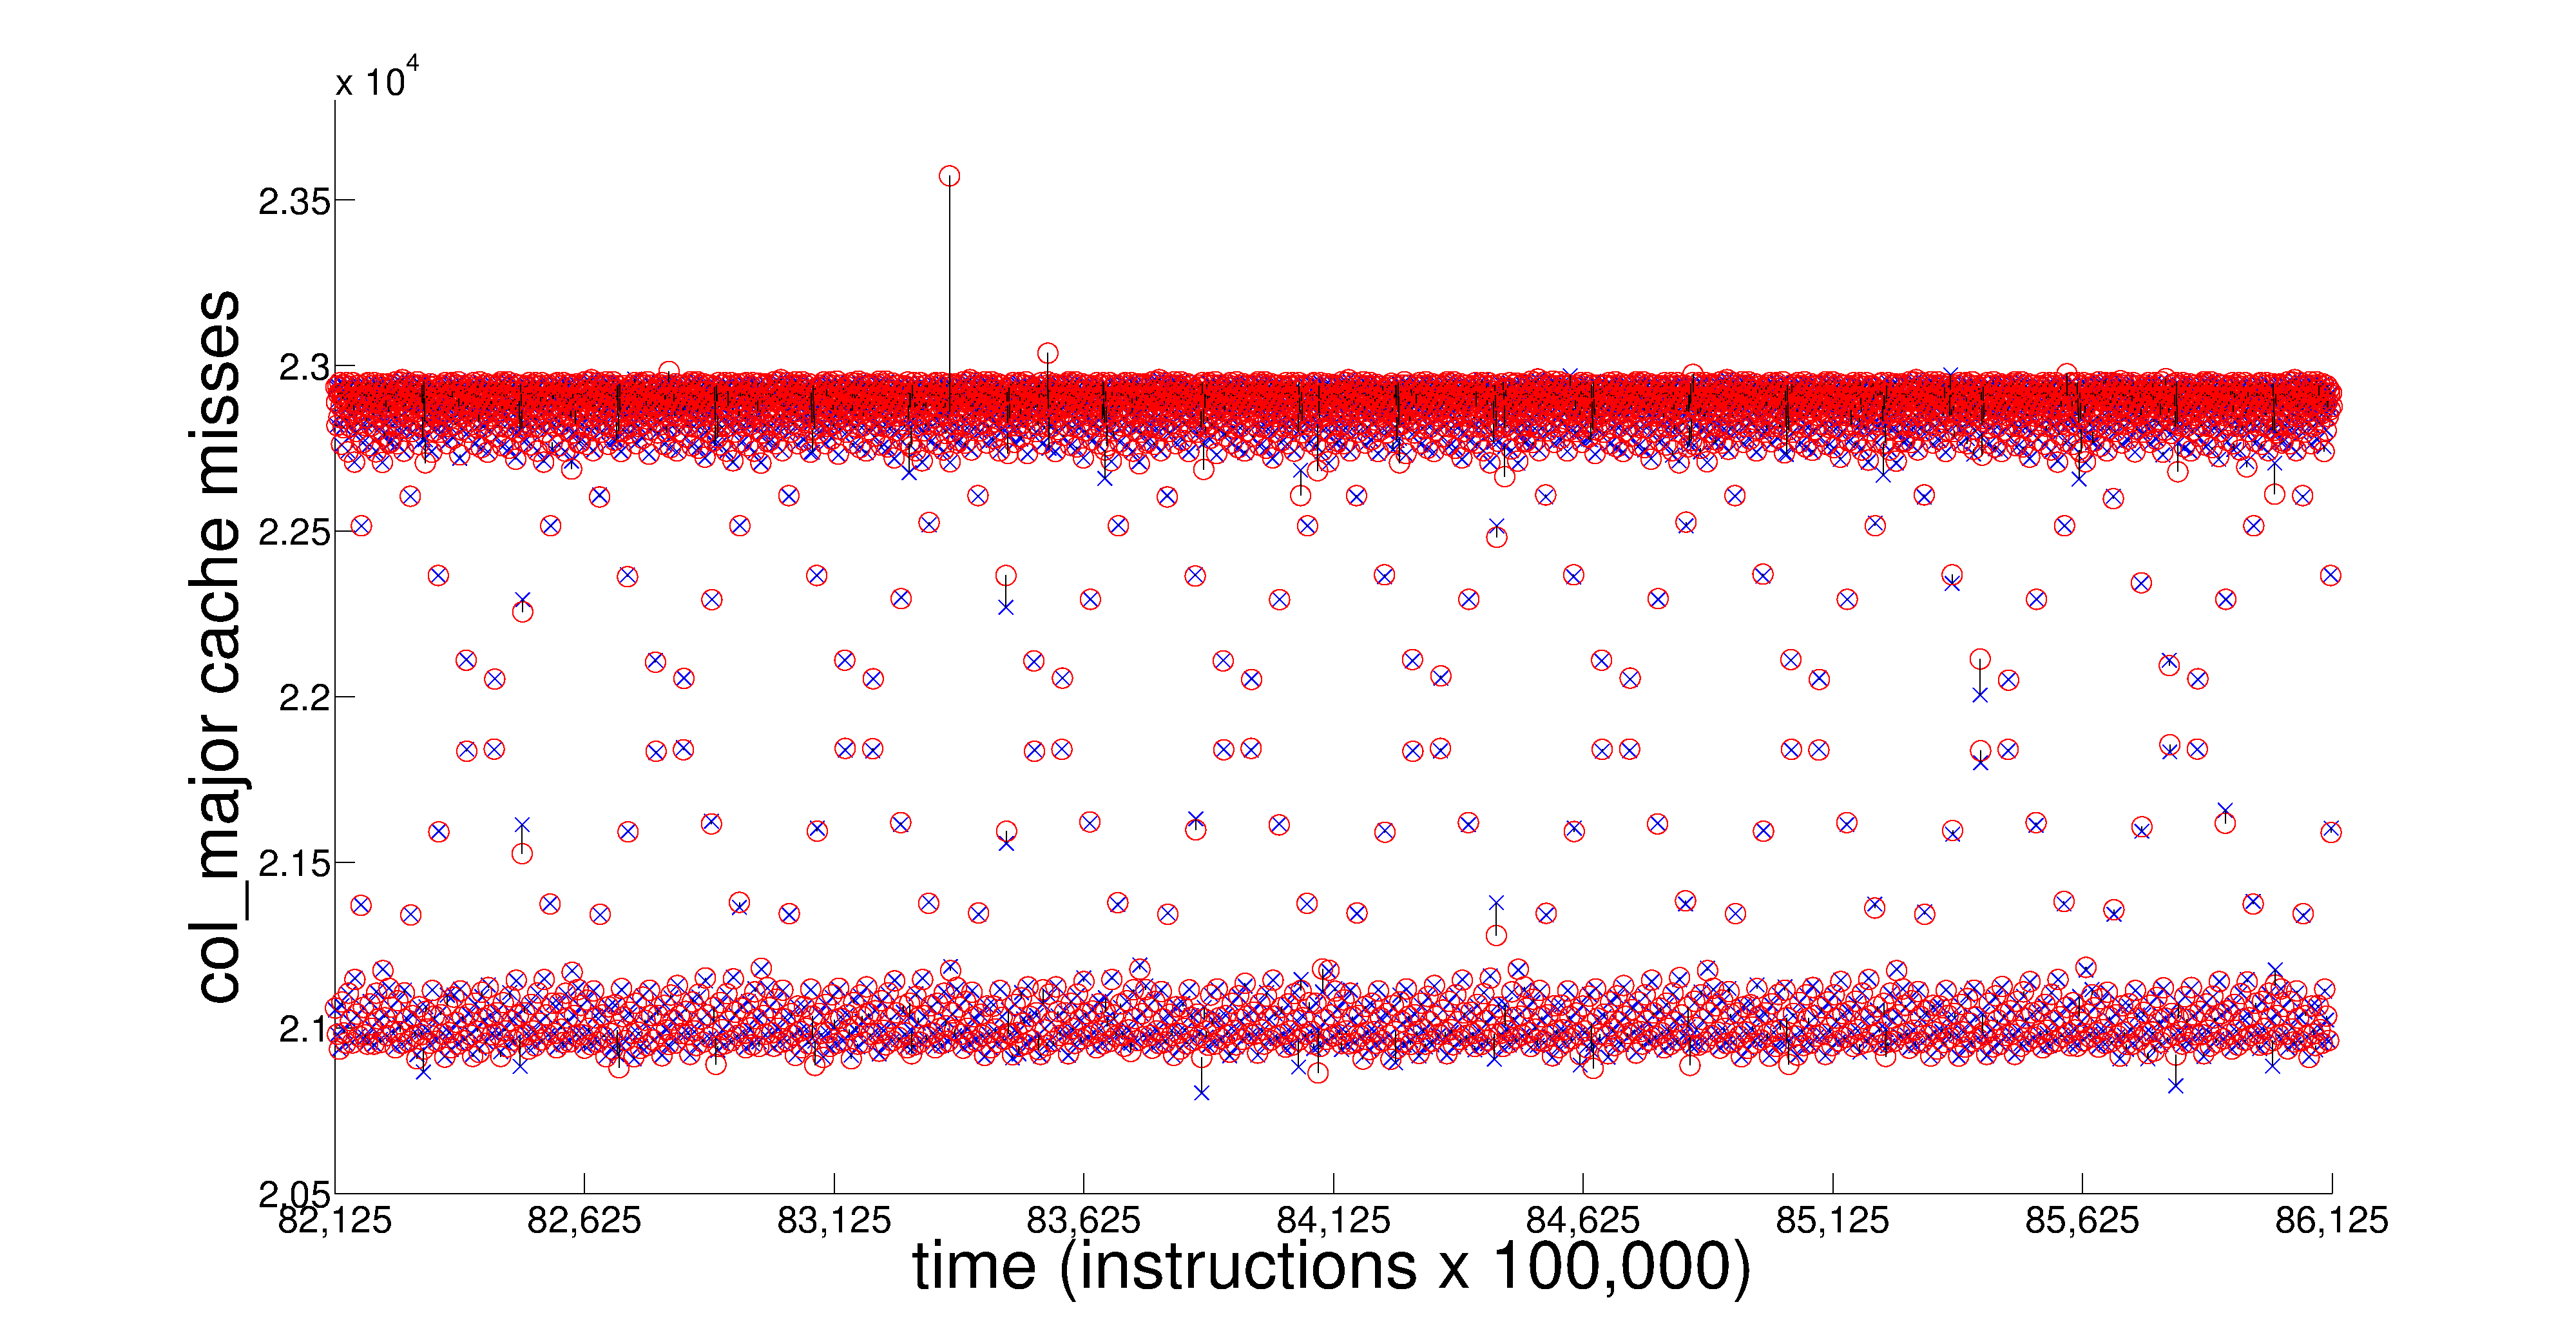
\includegraphics[width=0.5\textwidth]{figs/colCachePredTS}
    \caption{A forecast of the last 4,000 points of the signal in
      Figure~\ref{fig:ipc} using an LMA-based strategy on the
      embedding in Figure~\ref{fig:embedding}.  Red circles and blue
      $\times$s are the true and predicted values, respectively;
      vertical bars show where these values differ. }
\label{fig:cachePredTS}
\end{figure}
%
On the other hand, if we use the same approach to forecast the
processor load\footnote{Instructions per cycle, or IPC} of the {\tt
  482.sphinx3} program from the SPEC cpu2006 benchmark suite, running
on an Intel i7\textsuperscript{\textregistered}-based machine, the
prediction is far less accurate; see Figure~\ref{fig:predsphinx}.
%
\begin{figure}[htbp]
  \centering
    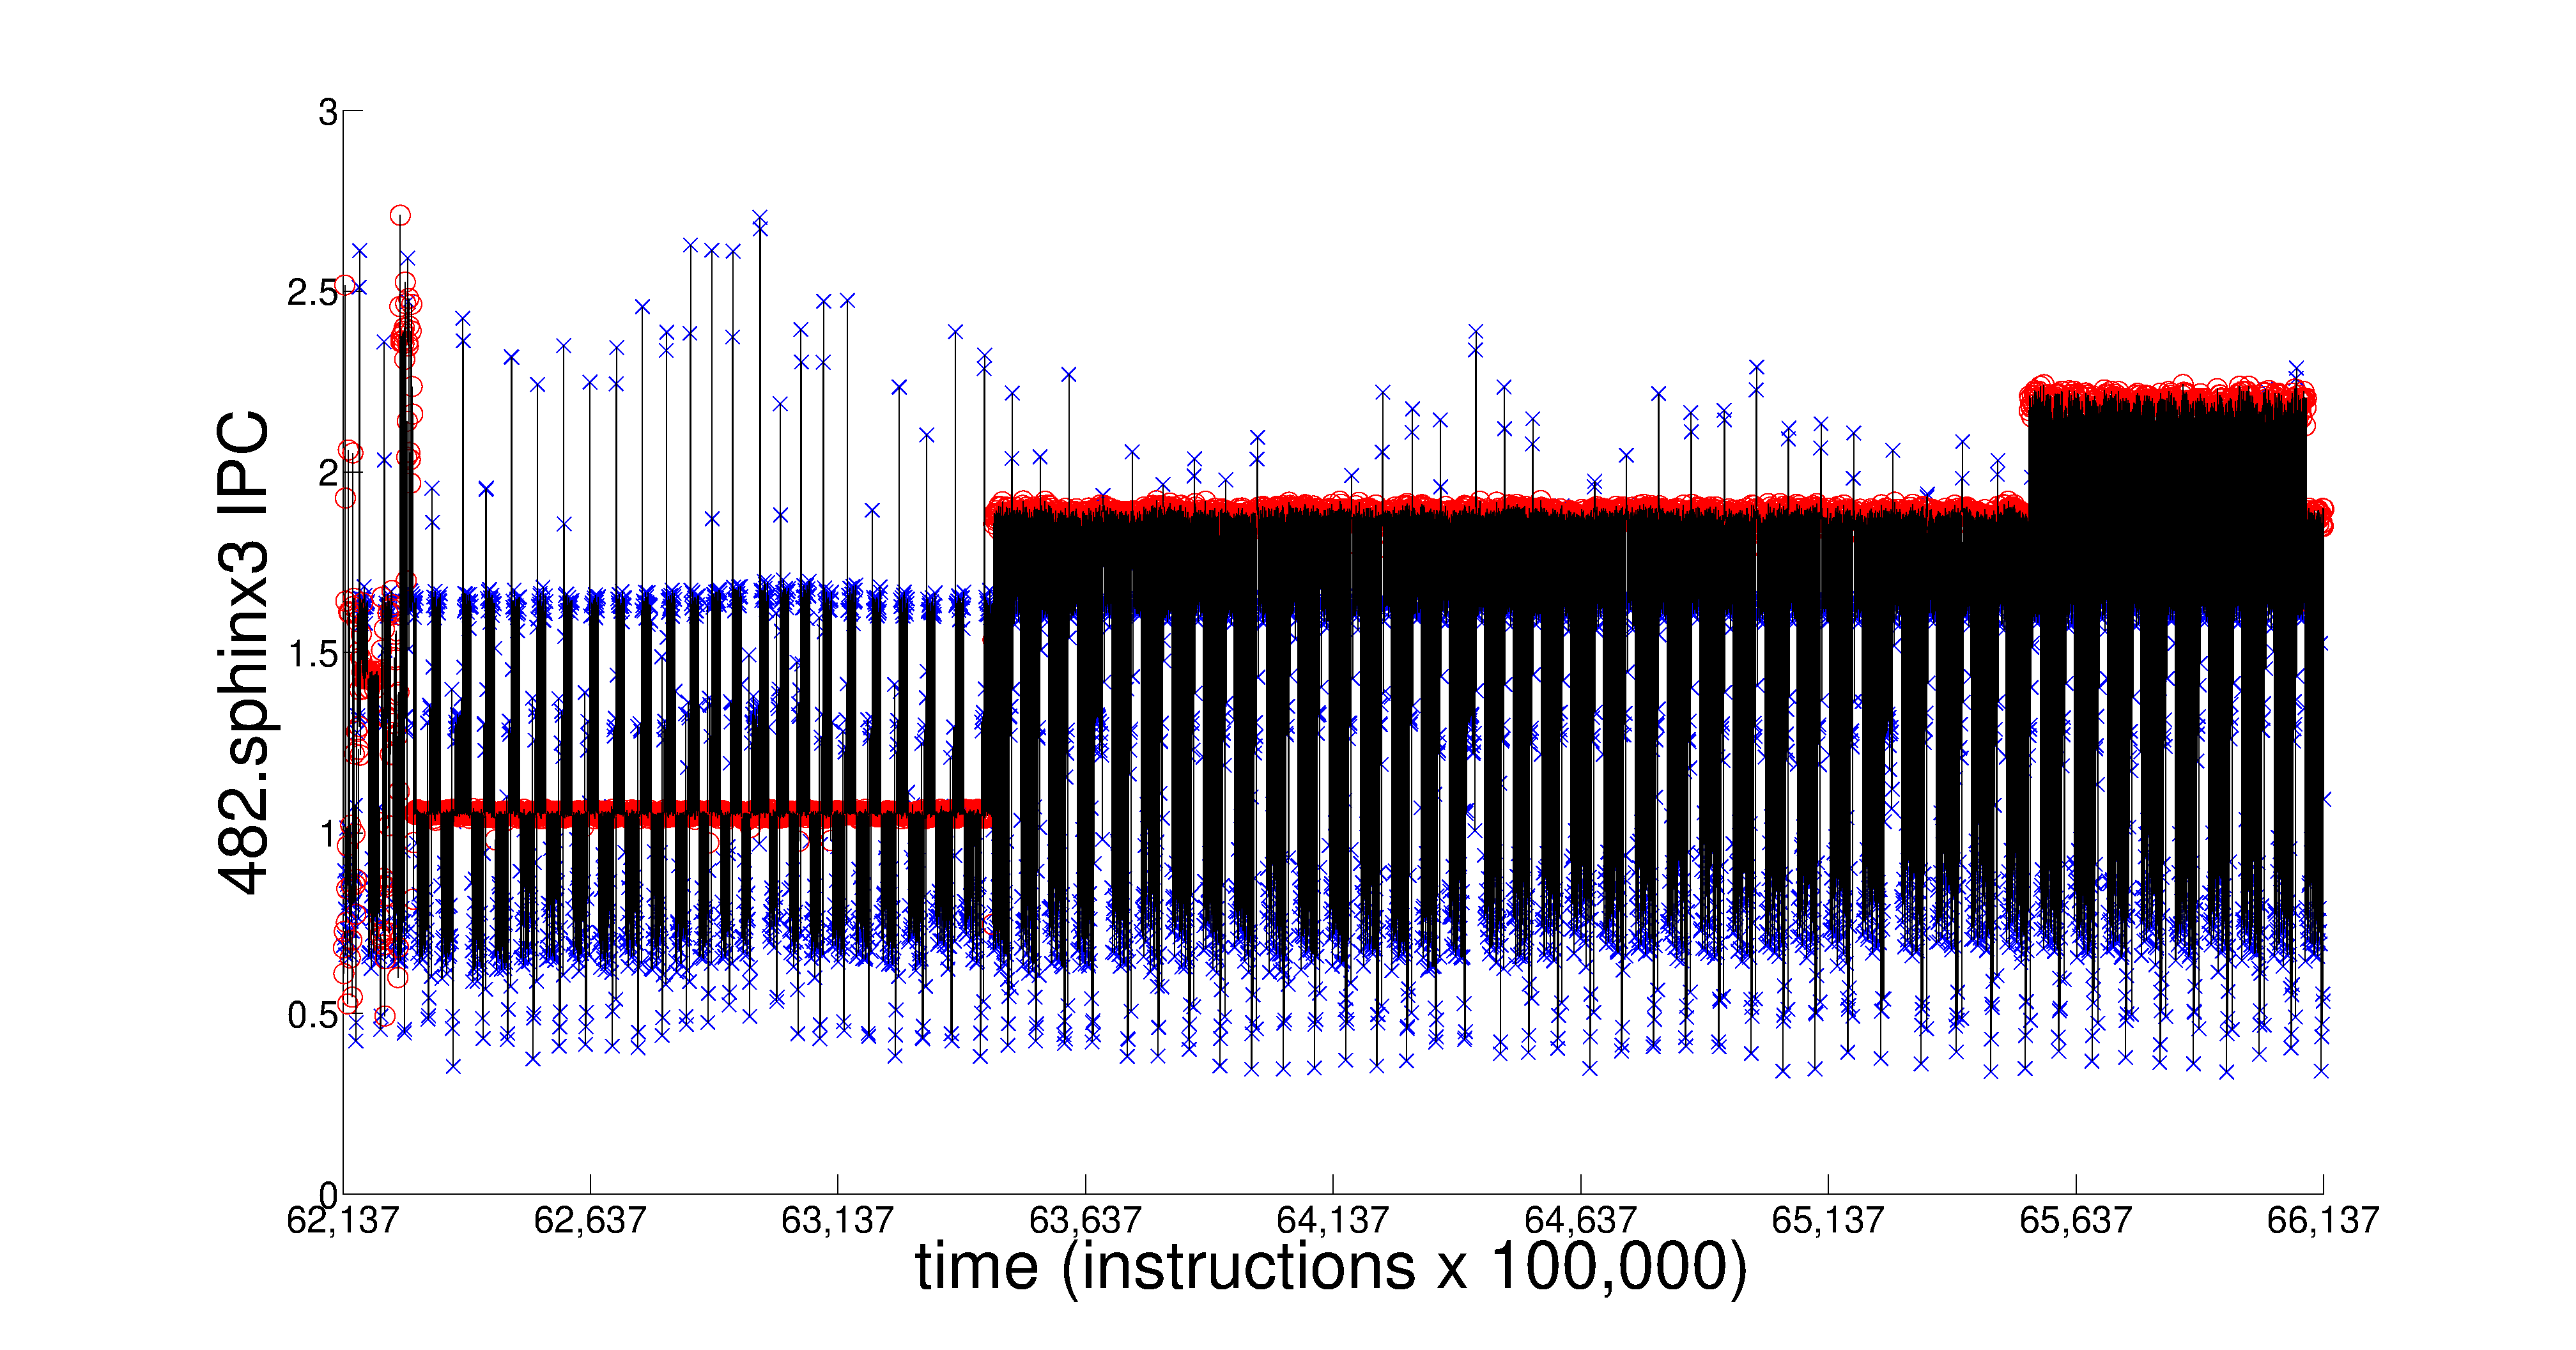
\includegraphics[width=0.5\textwidth]{figs/sphinxPredicTS}
     \caption{An LMA-based forecast of the last 4,000 points of a
       processor-load performance trace from the {\tt 482.sphinx3}
       benchmark.  Red circles and blue $\times$s are the true and
       predicted values, respectively; vertical bars show where these
       values differ.}
\label{fig:predsphinx}
\end{figure}

Table~\ref{tab:PredError} presents detailed results about the
prediction accuracy of this algorithm on four different examples: the
{\tt col\_major} and {\tt 482.sphinx3} programs in
Figures~\ref{fig:cachePredTS} and~\ref{fig:predsphinx}, as well as
another simple microkernel that initializes the same matrix as {\tt
  col\_major}, but in row-major order, and another complex program
({\tt 403.gcc}) from the SPEC cpu2006 benchmark suite.  Both
microkernels were run on the Intel Core
Duo\textsuperscript{\textregistered} machine; both SPEC benchmarks
were run on the Intel i7\textsuperscript{\textregistered} machine.  We
calculated a figure of merit for each prediction as follows.  We held
back the last $k$ elements\footnote{Several different prediction
  horizons were analyzed in our experiment; the results reported in
  this paper are for $k$=4000} of the $N$ points in each measured time
series, built the forecast model by embedding the first $N-k$ points,
used that embedding and the LMA method to predict the next $k$ points,
then computed the Root Mean Squared Error (RMSE) between the true and
predicted signals:
$$RMSE = \sqrt{\frac{\sum_{i=1}^k(c_i-\hat{p_i})^2}{k}}$$
%
To compare the success of predictions across signals with different
units, we normalized RMSE as follows:
$$nRMSE = \frac{RMSE}{X_{max,obs}-X_{min,obs}}$$
%
% The smaller the nRMSE, obviously, the more accurate the prediction.



The results in Table~\ref{tab:PredError} show a clear distinction
between the two microkernels, whose future behavior can be
predicted effectively using this simple deterministic modeling
strategy, and the more-complex SPEC benchmarks, for which this
prediction strategy does not work nearly as well.
% Removed for space
% For both processor load (IPC) and memory usage (cache-miss rate),
% forecasts for {\tt 482.sphinx3} and {\tt 403.gcc} are much worse than
% for \verb|col_major| or \verb|row_major|.
%
This begs the question: If these traces all come from deterministic
systems---computers---then why are they not equally predictable?  Our
conjecture is that the sheer complexity of the dynamics of the SPEC
benchmarks running on the Intel i7\textsuperscript{\textregistered}
machine make them effectively impossible to predict.

%% [[If space: Add a segue sentence: next section uses permutation
%% entropy to explore that conjecture.]]

\subsection{Comparing Prediction Accuracy}
In order to analyze correctness of each prediction we split each time series into two pieces: the first 90\% referred to as the ``learning" or ``training" signal, $\{X_{i,obs}\}_{i=1}^{n}$ and the last 10\% known as the ``test" or ``correct" signal $\{c_j\}_{j=n+1}^{k+n+1}$. The learning signal is used to train an initial model (e.g., LMA or ARIMA) as described in Section \ref{sec:compModel}. The test signal is used both to assess the models forecasting accuracy and for any refitting that may be necessary. In particular, we perform $k$ 1-step predictions, after each 1-step prediction we append the training signal with the next point in the correct signal $c_j$, refit the model taking into account the new system measurement and perform another prediction. This is repeated $k$ times to obtain $\{p_j\}_{j=n+1}^{k+n+1}$.\footnote{We would like to note that this rebuilding occurs due to a problem with ARIMA models converging to a mean prediction if too long of a prediction horizon is used, this is not a handicap of either LMA or na\"ive.}

As a figure of merit we calculate the Mean Absolute Squared Error (MASE)\cite{MASE} between the true and predicted signals: 
%In order to compare the resulting forecasts we calculate the Mean Absolute Squared Error (MASE)\cite{MASE} between the true and predicted signals:
$$MASE = \sum_{j=n+1}^{k+n+1}\frac{|c_j-p_j| }{\frac{k}{n-1}\sum^n_{i=2}|X_{i,obs}-X_{i-1,obs}|}$$
The scaling term for MASE:
$$\frac{1}{n-1}\sum^n_{i=2}|X_{i,obs}-X_{i-1,obs}|$$ 
is the average in-sample forecast error for a random walk prediction $(p_i=X_{i-1,obs})$. This error method was introduced in \cite{MASE} as a ``generally applicable measurement of forecast accuracy without the problems seen in the other measurements." The major advantage of MASE is that it allows fair comparison across methods, prediction horizons and varying signal scales. When a forecast results in a $MASE<1$ this means that the prediction method gave, on average, smaller errors than the 1-step errors from the in-sample random walk forecast strategy. Analogously, $MASE>1$ means that the prediction method did worse, on average than the 1-step errors for the in-sample random walk forecast strategy. In Table \ref{tab:error} we provide the distribution [[Joshua: Ryan, Is this the right word? we give mean $\pm$ std. dev but some have very skewed right tails]]  of MASEs for each of the 8 signals and 3 prediction strategies, these are averaged over 15 runs of each type (signal + method). For comparison Table \ref{tab:error} also has the distribution of weighted permutation entropies for word lengths of $l=5$ and $l=6$.


\begin{table}[htdp]
\caption{MASE distributions for 1-step predictions at a 10\% prediction horizon over 15 runs for each signal and average wpe at word length 5 and 6 for each signal.[[Joshua:Maybe delete $l=5$ as we don't use it in any figures, also if we leave this (before the next section we need to point forward to the next section for PE or remove it from this table]] }
\begin{center}
\begin{tabular}{|c|c|c|c|c|c|}
\hline
                   & MASE LMA    & MASE ARIMA &MASE na\"{i}ve & $l=5$  & $l=6$ \\
\hline
\gcc                  & $ 1.5296\pm 0.0214$ & $1.8366 \pm0.0157 $ & $1.7970\pm0.0095$& $0.9510 \pm 0.0011$ & $0.9430 \pm 0.0013$ \\

\col           & $ 0.0500 \pm0.0018  $ & $0.5989  \pm 0.2114 $ & $0.5707\pm0.0017$& $0.5636 \pm 0.0031$ & $0.5131 \pm 0.0034$ \\

\svd Reg. 1     & $ 0.8273\pm 0.0755$ & $ 0.7141\pm 0.0745 $ & $2.6763\pm4.3282$& $0.9761 \pm 0.0084$ & $0.9572 \pm 0.0156$ \\
\svd Reg. 2     & $1.2789 \pm0.0196 $ & $2.1626 \pm0.0265 $ &  $3.0543\pm0.0404$ &  $0.8760 \pm 0.0052$ & $0.8464 \pm0.0044$ \\
\svd Reg. 3       & $0.6192 \pm0.0209 $ & $0.7129 \pm 0.0096 $ & $31.3857\pm 0.2820$ & $0.7768 \pm 0.0073$ & $0.7157 \pm 0.0056$ \\
\svd Reg. 4     & $ 0.7789\pm0.0358 $ & $0.9787 \pm0.0321 $ & $2.6613\pm0.0739$                          &$0.9073 \pm 0.0080$ & $0.8246 \pm 0.0077$ \\
\svd Reg. 5     & $ 0.7177\pm 0.0483 $ & $2.3700  \pm 0.0505 $ & $20.8703 \pm 0.1915$& $0.7333 \pm 0.0076$ & $0.6776 \pm 0.0068$ \\
\svd Reg. 6     & $ 0.7393\pm 0.0682 $ & $ 1.4379\pm 0.0609$ & $2.1967\pm0.0830$& $0.8101 \pm 0.0135$ & $0.7475 \pm 0.0106$ \\
\hline
\end{tabular}
\end{center}
\label{tab:error}
\end{table}%




\section{Measuring Structural Complexity}\label{sec:meaComplex}

For the purposes of this paper, one can view entropy as a measure of complexity
and predictability in a time series.  A high-entropy time series is almost
completely unpredictable---and conversely.  This can be made more rigorous:
Pesin's relation \cite{pesin77} states that in chaotic dynamical systems, the
Shannon entropy rate is equal to the sum of the positive Lyapunov exponents,
$\lambda_i$. The Lyapunov exponents directly quantify the rate at which nearby
states of the system will diverge with time: $\left| \Delta x(t) \right| \approx
e^{\lambda t} \left| \Delta x(0) \right|$.  The faster the divergence, the more
difficult prediction becomes.

Utilizing entropy as a measure of temporal complexity is by no means a new idea
\cite{Shannon1951, mantegna1994linguistic}.  Its effective usage requires
categorical data: $x_t \in \mathcal{S}$ for some finite or countably infinite
\emph{alphabet} $\mathcal{S}$, whereas data taken from real-world systems is
effectively real-valued.  To get around this, one must discretize the data---
typically achieved by binning.  Unfortunately, this is rarely a good solution to
the problem, as the binning of the values introduces an additional dynamic on
top of the intrinsic dynamics whose entropy is desired.  The field of symbolic
dynamics studies how to discretize a time series in such a way that the
intrinsic behavior is not perverted, but these methods are fragile in the face
of noise and require further understanding of the underlying system, which
defeats the purpose of measuring the entropy in the first place.

Bandt and Pompe introduced the \emph{permutation entropy} (PE) as a ``natural
complexity measure for time series" \cite{bandt2002per}.  Permutation entropy
employs a method of discretizing real-valued time series that follows the
intrinsic behavior of the system under examination.  Rather than looking at the
statistics of sequences of values, as is done when computing the Shannon
entropy, permutation entropy looks at the statistics of the \emph{orderings} of
sequences of values using ordinal analysis. Ordinal analysis of a time series is
the process of mapping successive time-ordered elements of a time series to
their value-ordered permutation of the same size.  By way of example, if $(x_1,
x_2, x_3) = (9, 1, 7)$ then its \emph{ordinal pattern}, $\phi(x_1, x_2, x_3)$,
is $231$ since $x_2 \leq x_3 \leq x_1$.  This method has many features; among
other things, it is generally robust to observational noise and requires no
knowledge of the underlying mechanisms.

\begin{mydef}[Permutation Entropy]

  Given a time series $\{x_t\}_{t = 1,\dots,T}$. Define $\mathcal{S}_n$ as all
  $n!$ permutations $\pi$ of order $n$. For each $\pi \in \mathcal{S}_n$ we
  determine the relative frequency of that permutation occurring in $\{x_t\}_{t
  = 1,\dots,T}$:
  \begin{align*}
    p(\pi) = \frac{\left|\{t|t \leq T-n,\phi(x_{t+1},\dots,x_{t+n}) = \pi\}\right|}{T-n+1}
  \end{align*}
  Where $|\cdot|$ is set cardinality. The \emph{permutation entropy} of order $n
  \ge 2$ is defined as
  \begin{align*}
  H(n) = - \sum_{\pi \in \mathcal{S}_n} p(\pi) \log_2 p(\pi)
  \end{align*}

\end{mydef}

Notice that $0\le H(n) \le \log_2(n!)$ \cite{bandt2002per}.  With this in mind,
it is common in the literature to normalize permutation entropy as follows:
$\frac{H(n)}{\log_2(n!)}$.  With this convention, ``low'' entropy is close to 0
and ``high'' entropy is close to 1. Finally, it should be noted that the
permutation entropy has been shown to be identical to the Shannon entropy for
many large classes of systems \cite{amigo2012permutation}.

Here we will be utilizing a variation of the permutation entropy, the
\emph{weighted permutation entropy} (WPE)~\cite{fadlallah2013}. The weighted
permutation entropy attempts to correct for observational noise which is larger
than some trends in the data, but smaller than the larger scale features --- for
example, a signal that switches between two fixed points with noise about those
fixed points. The weighted permutation entropy would be dominated by the
switching rather than by the stochastic fluctuation. To accomplish this, the
\emph{weight} of a permutation is taken into account:
\begin{align*}
  w(x_{t+1:t+n}) = \frac{1}{n}
                 \sum_{x_i \in \{x_{t+1:t+n}\}}
                 \left( x_i - \bar{x}_{t+1:t+n} \right)^2
\end{align*}
where $x_{t+1:t+n}$ is a sequence of values $x_{t+1}, \ldots, x_{t+n}$, and
$\bar{x}_{t+1:t+n}$ is the arithmetic mean of those values.

The weighted probability of a permutation is then:
\begin{align*}
  p_w(\pi) = \frac{\displaystyle \sum_{t \le T - n} w(x_{t+1:t+n}) \cdot \delta(\phi(x_{t:t+n}), \pi) }{\displaystyle \sum_{t \le T - n} w(x_{t+1:t+n})}
\end{align*}
where $\delta(x, y)$ is 1 if $x = y$ and 0 otherwise. Effectively, this weighted
probability enhances permutations involved in ``large'' features and demotes
permutations which are small in amplitude relative to the features of the time
series. The weighted permutation entropy is then:
\begin{align*}
  H_w(n) = - \sum_{\pi \in \mathcal{S}_n} p_w(\pi) \log_2 p_w(\pi),
\end{align*}
which can also be normalized by dividing by $\log_2(n!)$, and will be in all the
results of this paper.

In practice, calculating permutation entropy and weighted permutation entropy
involves choosing a good value for the word length $n$. The primary
consideration is that the value be large enough that forbidden ordinals are
discovered, yet small enough that reasonable statistics over the ordinals are
gathered: e.g.:
\begin{align*}
  n = \operatornamewithlimits{argmax}_\ell \{ T \gtrapprox 100 \ell! \},
\end{align*}
assuming an average of 100 counts per ordinal is sufficient. In the literature,
$3 \le n \le 6$ is a standard choice --- generally without any formal
justification. In theory, the permutation entropy should reach an asymptote with
increasing $n$, but that requires an arbitrarily long time series. In practice,
what one should do is calculate the \emph{persistent} permutation entropy by
increasing $n$ until the result converges, but data length issues can intrude
before that convergence is reached.

The weighted permutation entropy for the {\tt SVD} program is given in
Fig.~\ref{fig:wwpe}. To generate this image a window of 5,000 values slid over
the time series. Within each of those windows, the statistics over words of
length 4 are computed and the WPE is calculated. The gray bands denote regions
where the 5,000 value window overlapped visually-distinct regimes. It can be
seen that the behaviors of the weighted permutation entropy vary between
regimes. [[I think here it would be good to add a paragraph explaining the windowed WPE was used for regime choices on SVD...emphasizing  that over a time series permutation entropy fluctuates illustrating within a single time series different levels of complexity and predictability exist. Maybe point at some of the predicting predictability papers.]]

%\begin{figure}[htbp]
%  \centering
%  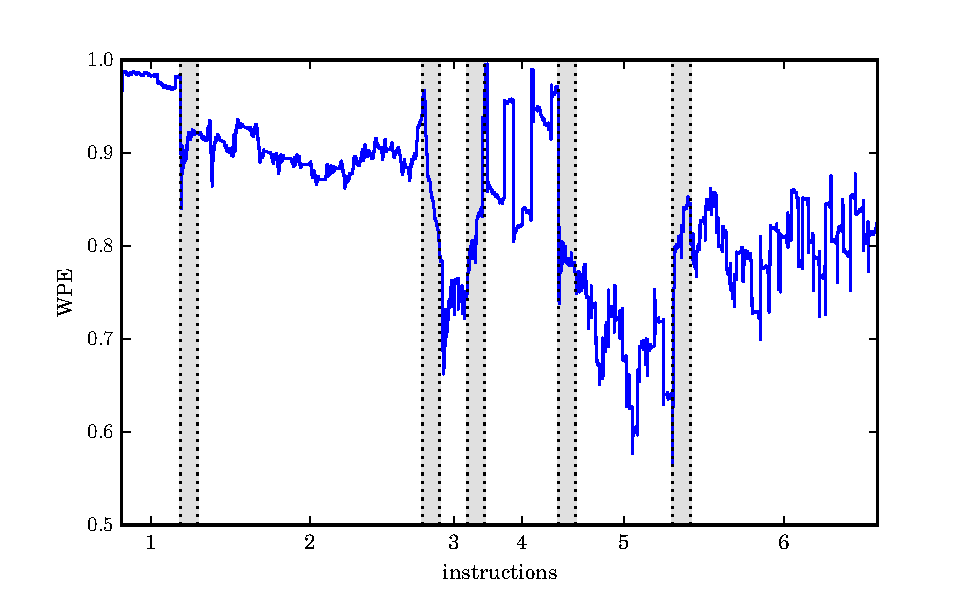
\includegraphics[width=1.0\textwidth]{figs/SVD_wwpe}
%  \caption{[[Joshua: I think adding the colored SVD trace to this would be %good or putting it above this figure]]The weighted permutation entropy of %one run of SVD. The gray bands
%    are regions where the window overlaps regimes. The window size used is
%    $5,000 \times 100,000$ instructions and the word length is $4$.}
%  \label{fig:wwpe}
%\end{figure}


%%FIGURE INTENT
%This figure shows that entropy changs over time with the signal as well as why the regimes for \svd were chosen. 
%%%%%%%%%%%%%%%%%
\begin{figure}[htbp]
  \centering
         \caption{
[Joshua: I think adding the colored SVD trace to this would be good or putting it above this figure but need to figure how to line them up properly. Also we need to label that the numbers on the bottom of WPE are regimes not instructions...]]The weighted permutation entropy of one run of SVD. The gray bands
    are regions where the window overlaps regimes. The window size used is
    $5,000 \times 100,000$ instructions and the word length is $4$.}\label{fig:wwpe}
  \begin{subfigure}{0.3\textwidth}
    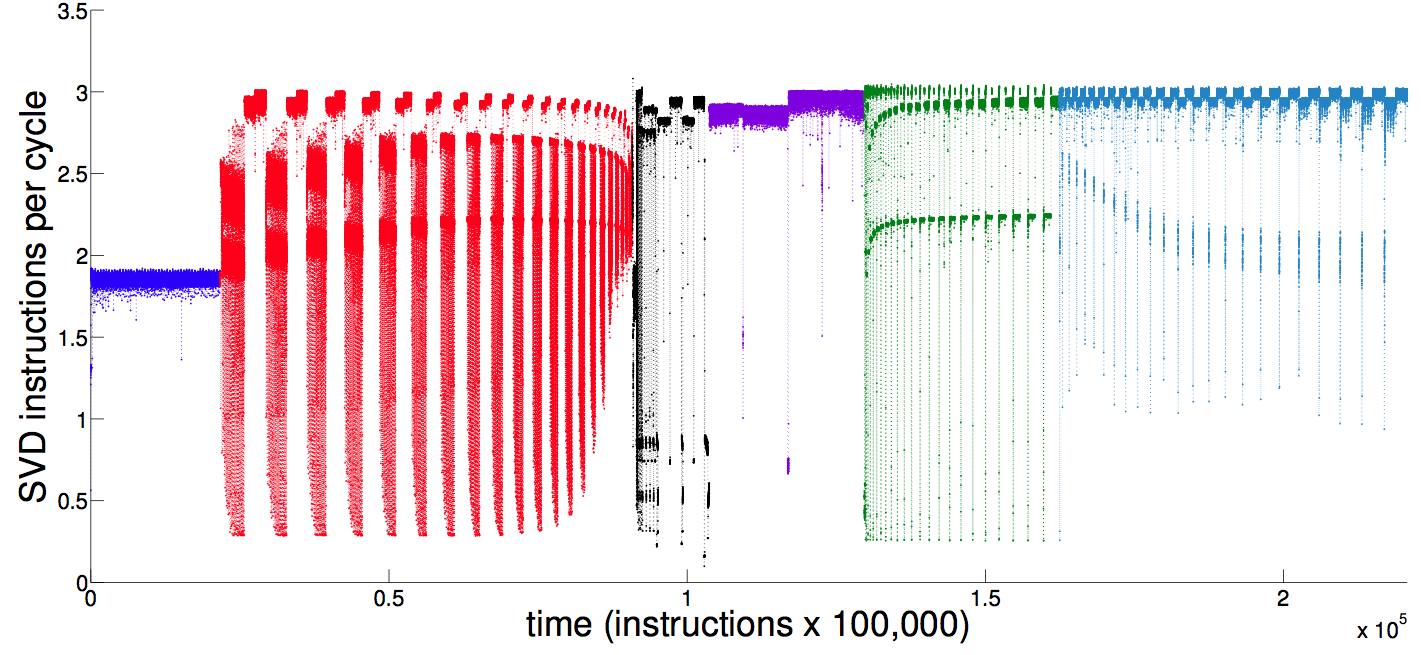
\includegraphics[width=0.3\textwidth]{figs/svdipcregimescolored.png}
    \caption{The instructions per cycle of \svd. Each color corresonds to the different regimes as selected by rapid shifts in WPE, as seen in Figure \ref{fig:svd_wwpe}. From left to right each change in color represents a change in regime for 6 regimes in total. }
    \label{fig:svd_ts}
  \end{subfigure}%
  %\\
  \begin{subfigure}{\textwidth}
    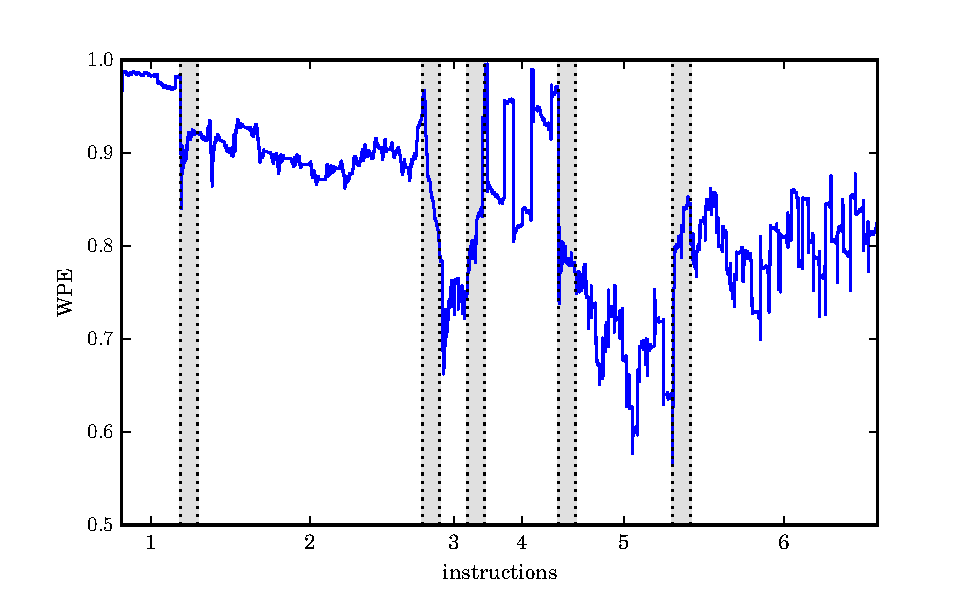
\includegraphics[width=\textwidth]{figs/SVD_wwpe}
    \caption{The MASE of ARIMA vs weighted permutation entropy. }
    \label{fig:svd_wwpe}
  \end{subfigure}
  %\begin{subfigure}{0.5\textwidth}
  %  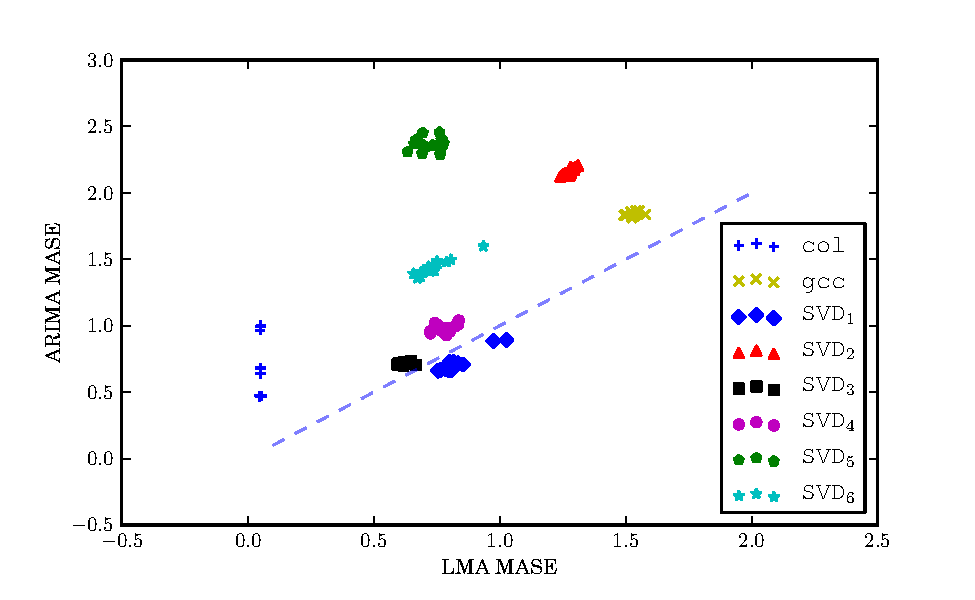
\includegraphics[width=1.0\textwidth]{figs/LMA_vs_ARIMA}
   % \caption{The MASE values for LMA against ARIMA. The dashed line is the
   % identity, delineating the traces for which either LMA or ARIMA %performed
%    better. All traces except those from {\tt SVD$_1$} lie above the line,
%    indicating that LMA is better suited prediction method for the %computer
%   traces considered.}\label{fig:lma_vs_arima}
  %\end{subfigure}
\end{figure}






 \section{Validation of Primary Findings} % (fold)
 \label{sec:results}


OUTLINE:
\begin{enumerate}
\item \cmark~Introduce MASE.
\item \cmark~WPE is a good measure of predictability.  Figure: best athlete MASE vs.
its WPE.
\item \cmark~Talk about structure analysis. Just because there is forward information
transfer, does not mean that linear predictors can get at this.
\subitem \cmark~For this show a figure of (a) ARIMA vs MASE (b) LMA vs MASE in a side by
side plot.
\item full results.  Image: MASE vs. WPE for both LMA \& ARIMA.  Points to make:
\begin{enumerate}
\item \cmark~clusters are distributed differently
\item \cmark~clusters are shaped differently---tight or not
\item \cmark~clusters move differently between LMA and ARIMA
\item finally, the diagonal line is important. If you're below it, you could do
better.
\end{enumerate}
\end{enumerate}

BRAINSTORMING 
\begin{itemize}
\item Complexity need not be hard to predict (can point at the simple predictions paper) [[move to introduction]]
\item random walk for example is best predicted by guess what just happend[[move to introduction]]
\item The kind of complexity present matters, i.e., that is whether the complexity is structured or not.[[use here and mention in intro]] 
\item Quantifying structured and unstructured complexity is nontrivial in the case of real-valued noisy time series but WPE does this. [[talk about again here but justify in information theory section]]
%\item Maybe plot a big chunk of \col and a big chunk of \gcc together and show that they both look complex. 

\item \gcc appears visually very complex, *and* according to WPE this complexity is unstructured. And a constant, linear and nonlinear prediction strategy all fail. We should be able to conclude that guessing random values is the best we can do as is shown by MASE [[Use in this section]]

\item \col is also complex (can even be chaotic/ point to CHAOS paper) but the complexity is structured according to WPE and as such that complexity is usable for prediction [[use in this section]]

\item \col brings about the point nicely that some prediction strategies cannot utilize the processes internal information transfer method. That is a nonlinear internal information transfer system cannot be predicted effectively with a linear strategy. This gives a practitioner leverage on when to give up and when to keep working. [[use in this section as bridge to next section]]

\end{itemize}


In this section we validate the two key primary findings of this work which we introduced in Section \ref{sec:intro}:



\begin{enumerate}

\item The existence of predictable structure in noisy real-valued time series is quantifiable by WPE and as a result WPE is correlated with prediction accuracy (MASE) of an ideal predictor. 

\subitem [[Simply reminders not to be included]]WPE can quantify when a noisy real-valued time series is predictable.[[I am unsatisfied with predictable in this sentence, need a better word to say "better than random walk" or ``able to be forecast effectively" or ``has the structural capacity to transmit information in a way that the time series can be effectively forecast"

%\item The existence of complex structure in a noisy real-valued time series is quantifiable and this type of complexity is directly correlated with predictability

\item The way structure/information/complexity is processed internally by a given process plays a crucial role in predictability.


\subitem [[Simply reminders not to be included]]We will have shown that the existence whether linear or nonlinear is picked up on with WPE but this point gets at whether the prediction model can use the structure or not (linear can't use nonlinear structure). The right to left shifts in \col and some of the \svd regimes and the lack of shift in \gcc illustrate this nicely.

\subitem [[Simply reminders not to be included]]This is the linear vs nonliear vs random we see with the right to left shifts with lower complexity time series. 

 
\end{enumerate}



%This portion should justify the following claim%%%%%%%%%%%%%%%%%%%%%%
%\item The existence of predictable structure in noisy real-valued time series is quantifiable by WPE and as a result WPE is correlated with prediction accuracy (MASE)  
%%%%%%%%%%%%%%%%%%%%%%%%%





%\item First paragraph: WPE is a good measure of predictability.  Figure:
%best athlete MASE vs. its WPE. 


%\item Quantifying structured and unstructured complexity is nontrivial in the case of real-valued noisy time series but WPE does this. [[talk about again here but justify in information theory section]]

As we discussed in Section \ref{sec:meaComplex} distinguishing structured from unstructured complexity in the case of real-valued time series is non trivial, i.e., distinguishing when a complex signal omits predictable structure and when the signal is effectively random is not a trivial task. As described in Section \ref{sec:intro}, for a practitioner this can be frustrating because it can be nearly impossible to find the source of faulty predictions: Is it simply that we need to use a more ideal (possibly more advanced) predictor or is it the case that the time series is simply so complex that using a simple (yet inconsistent) forecast strategy such as random walk is the best we can do. Fortunately, weighted permutation entropy (WPE) allows us to make this distinction for noisy real-valued time series. 

In Figure~\ref{fig:pred_vs_wpe} we plot the best prediction (i.e., the lowest MASE over all 3 methods\footnote{LMA,ARIMA,na\"ive} over all 15 runs of that program) for each of the 8 programs under investigation. 
\begin{figure}[htbp]
  \centering
  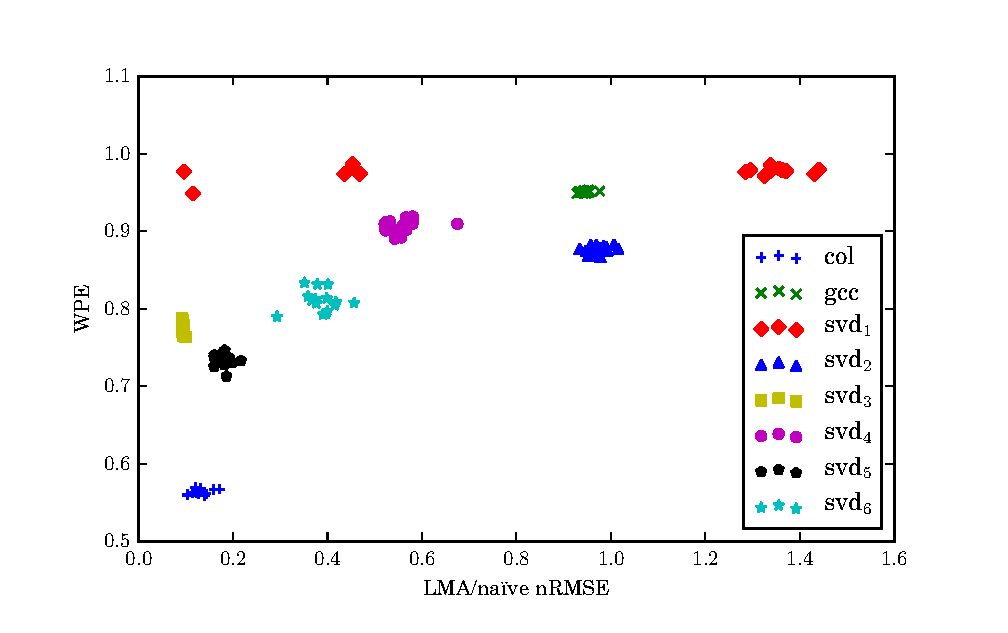
\includegraphics[width=0.75\textwidth]{figs/prediction_vs_entropy}
  \caption{The best MASE among all runs and prediction methods vs weighted
  permutation entropy. For each of these, the word length used is $6$. The
  dashed line is a least-squares linear fit of all the points except for {\tt
  SVD$_1$} which we have excluded for reasons explained in the text.}
  \label{fig:pred_vs_wpe}
\end{figure}
What we see here is that the relationship between prediction accuracy (MASE) and the weighted permutation entropy is much as we conjectured: The existence of predictable structure in noisy real-valued time series as quantified by low to moderate WPE  is correlated with prediction accuracy (MASE) of the ``best"predictor\footnote{We do not claim to have found the ideal predictor for each signal, simply the best predictor over what we used; Which we believe to be a fair sampling of standard prediction techniques for this type of signal.}. We will not further validate this claim through some examples. 


To further validate this finding we present an in-depth analysis of three examples (\col, \svdfive and \gcc ) which nicely cover the range of complexity from low to high respectively. In Figures~\ref{fig:lma_vs_arima} and \ref{fig:arima_pred_vs_ent} we plot the MASE of LMA and ARIMA (respectively) against the weighted permutation entropy of each of the 15 runs of all 8 programs.


\begin{figure}[htbp]
  \centering
       
  \begin{subfigure}{0.5\textwidth}
    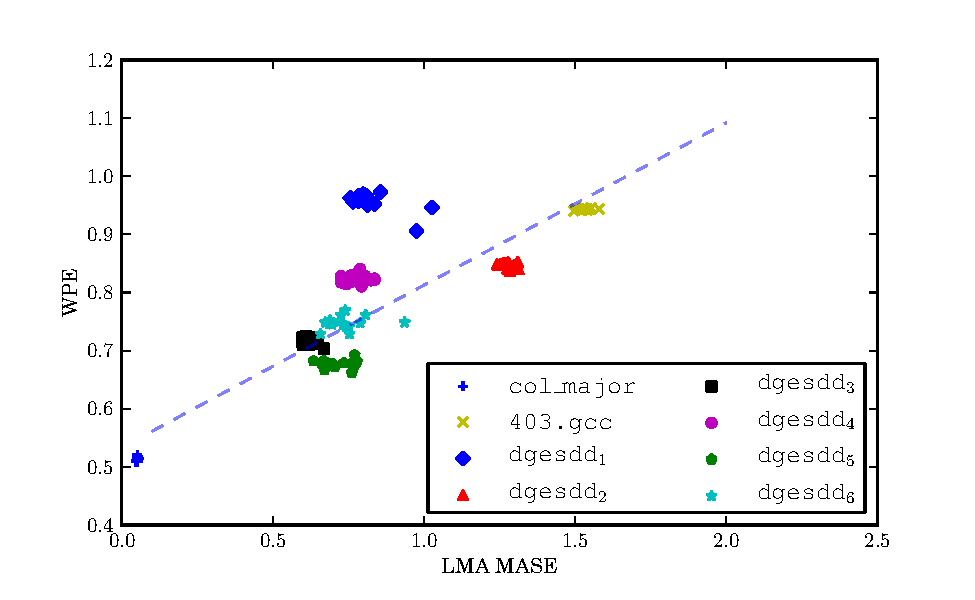
\includegraphics[width=\textwidth]{figs/LMA_prediction_vs_entropy}
    \caption{The MASE of LMA vs weighted permutation entropy. }
    \label{fig:lma_pred_vs_ent}
  \end{subfigure}%
  \begin{subfigure}{0.5\textwidth}
    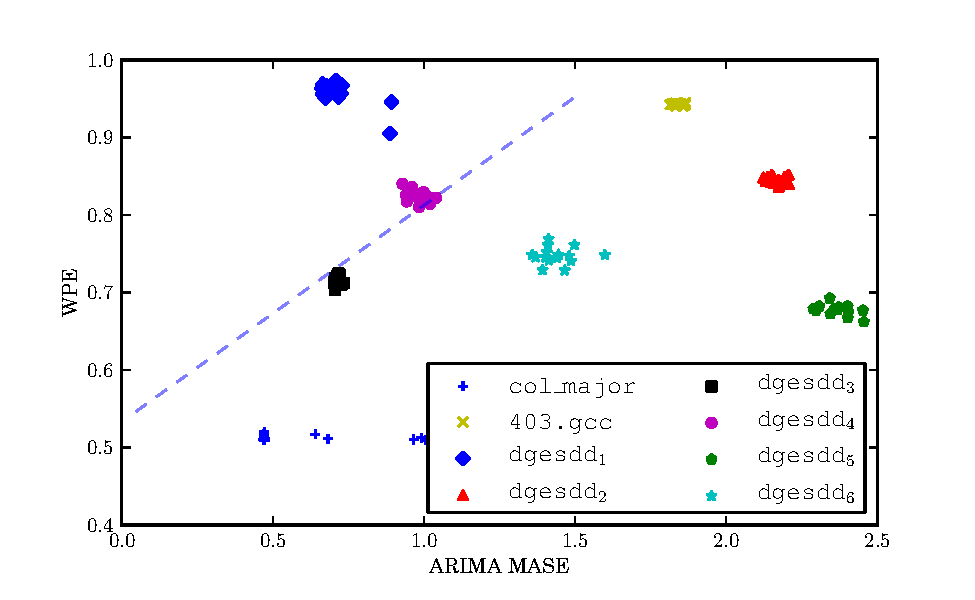
\includegraphics[width=\textwidth]{figs/ARIMA_prediction_vs_entropy}
    \caption{The MASE of ARIMA vs weighted permutation entropy. }
    \label{fig:arima_pred_vs_ent}
  \end{subfigure}
\caption{
For each of these, the word length used is $6$. The MASE values for LMA against ARIMA. The dashed line is the identity, delineating the traces for which either LMA or ARIMA performed better. All traces except those from \svd$_1$ lie above the line, indicating that LMA is better suited prediction method for the computer traces considered.}\label{fig:lma_vs_arima}  
\end{figure} 

We will start with the lowest complexity program: \col. Conceptually this program is very simple but due to computer design choices this program can result in highly complex even chaotic time series traces, see \cite{mytkowicz09}. If we forecast this signal using an out-of-the-box linear forecaster (ARIMA) or an out-of-the-box constant predictor we receive MASE ($0.59 \pm 0.21$ and $0.57 \pm$ 0.001 respectively) which suggest that on average we can only predict this signal twice as well as the simple random walk prediction. This would suggest that there is some predictive structure present but not that much. However, if we quantify the predictive structure present in this signal using WPE we see that this signal is highly structured with a WPE of ($0.51 \pm 0.003$.) The existence of structured which we quantified with WPE implies that an ideal predictor capable of using this signals information should be able to predict this signal much better than the random walk due to the high amount of predictive structure or equivalently the low complexity. This is in fact the case. \col is a complex signal, i.e., chaotic, but it is complex in a structured way. Using a prediction technique that can process nonlinear information yields forecasts with a MASE of $0.05 \pm 0.001$, this is a prediction 20 times more accurate than a random walk forecast. The existence of predictive structure as quantified by WPE could be precisely the information needed to continue searching for an ideal predictor like LMA. 

Maybe even more convincing than a low complexity signal like \col is a moderately complex signal like \svdfive. This signal omits a WPE of $0.677 \pm 0.006$, this is a significantly higher complexity than \col but still implies the existence of a great deal of predictive structure. However, this increase in complexity is enough to really throw off the constant and linear prediction strategies. The MASE scores for ARIMA and na\"ive imply 2.5 and 20 times worse prediction than using a simple random walk forecast. This may be discouraging to someone using an out-of-the-box predictor that the signal is too complex to predict. However by \emph{knowing} that there exists predictable  in this signal we can try to use a more advanced technique, in particular LMA. If we do this we get forecasts which score 1.5 times better than the random walk. Showing that this usable structure (although hidden to the linear and constant method) was quantifiable by WPE.

Finally, we consider the most complex program: \gcc. The complexity of \gcc is $0.94 \pm 0.001$. This implies that almost no predictive structure exists in this structure. Recall that a WPE $\approx 1$ are similar in complexity to white noise or a random walk process as they do not transmit any information from past to future. This would mean that the WPE of $>0.95$ would suggest little to no predictive structure exists and that the signal is simply too complex. In this case it should be safe to assume that a random walk forecast would be (on-average) superior to forecast methods which required structure or information to intelligently predict the next time step. This is in fact what we see, with each prediction scheme we used we see a MASE which implies (on-average) 1.5-1.8 times worse predictions that performing a simple random walk forecast. 

There is a single outlier in this study which is \svdone. This signal has a WPE of $0.95 \pm 0.02$ and both LMA and ARIMA do slightly better than random walk ($0.82 \pm 0.08$ and $0.7141 \pm 0.07$ respectively). The na\"ive method did significantly worse than random walk and was highly inconsistent with an average MASE of 2.67 but a standard deviation of 4.33 due to the massive right tail this distribution exhibited in reaction to wildly inconsistent forecasts. We do not believe this outlier is really a problem but it does bring about a potential weaknesses of this method. MASE is scaled by a random walk forecast which can be very inconsistent in the case of drastic signal changes which occur on a regular basis, e.g., a signal which oscillates from the top to the bottom of the signals scale at every time click. In this case a random walk forecast would have error with magnitude of the scale of the signal at every forecast, since guessing the last step will be exactly out of phase with the new forecast. A signal like this would normally cause a very low WPE much like \col and a very high Random Walk error resulting in low MASE for methods that can take into account this structure like ARIMA or LMA. 

To understand why this causes \svdone to be an outlier we examine Figure \ref{fig:svdone-ts} in more detail. This is a small snippet of the time series of \svdone to illustrate the strucutre of this signal. We provide a small snippet as opposed to the full time series simply for visual clarity.
\begin{figure}[htbp]
  \centering
    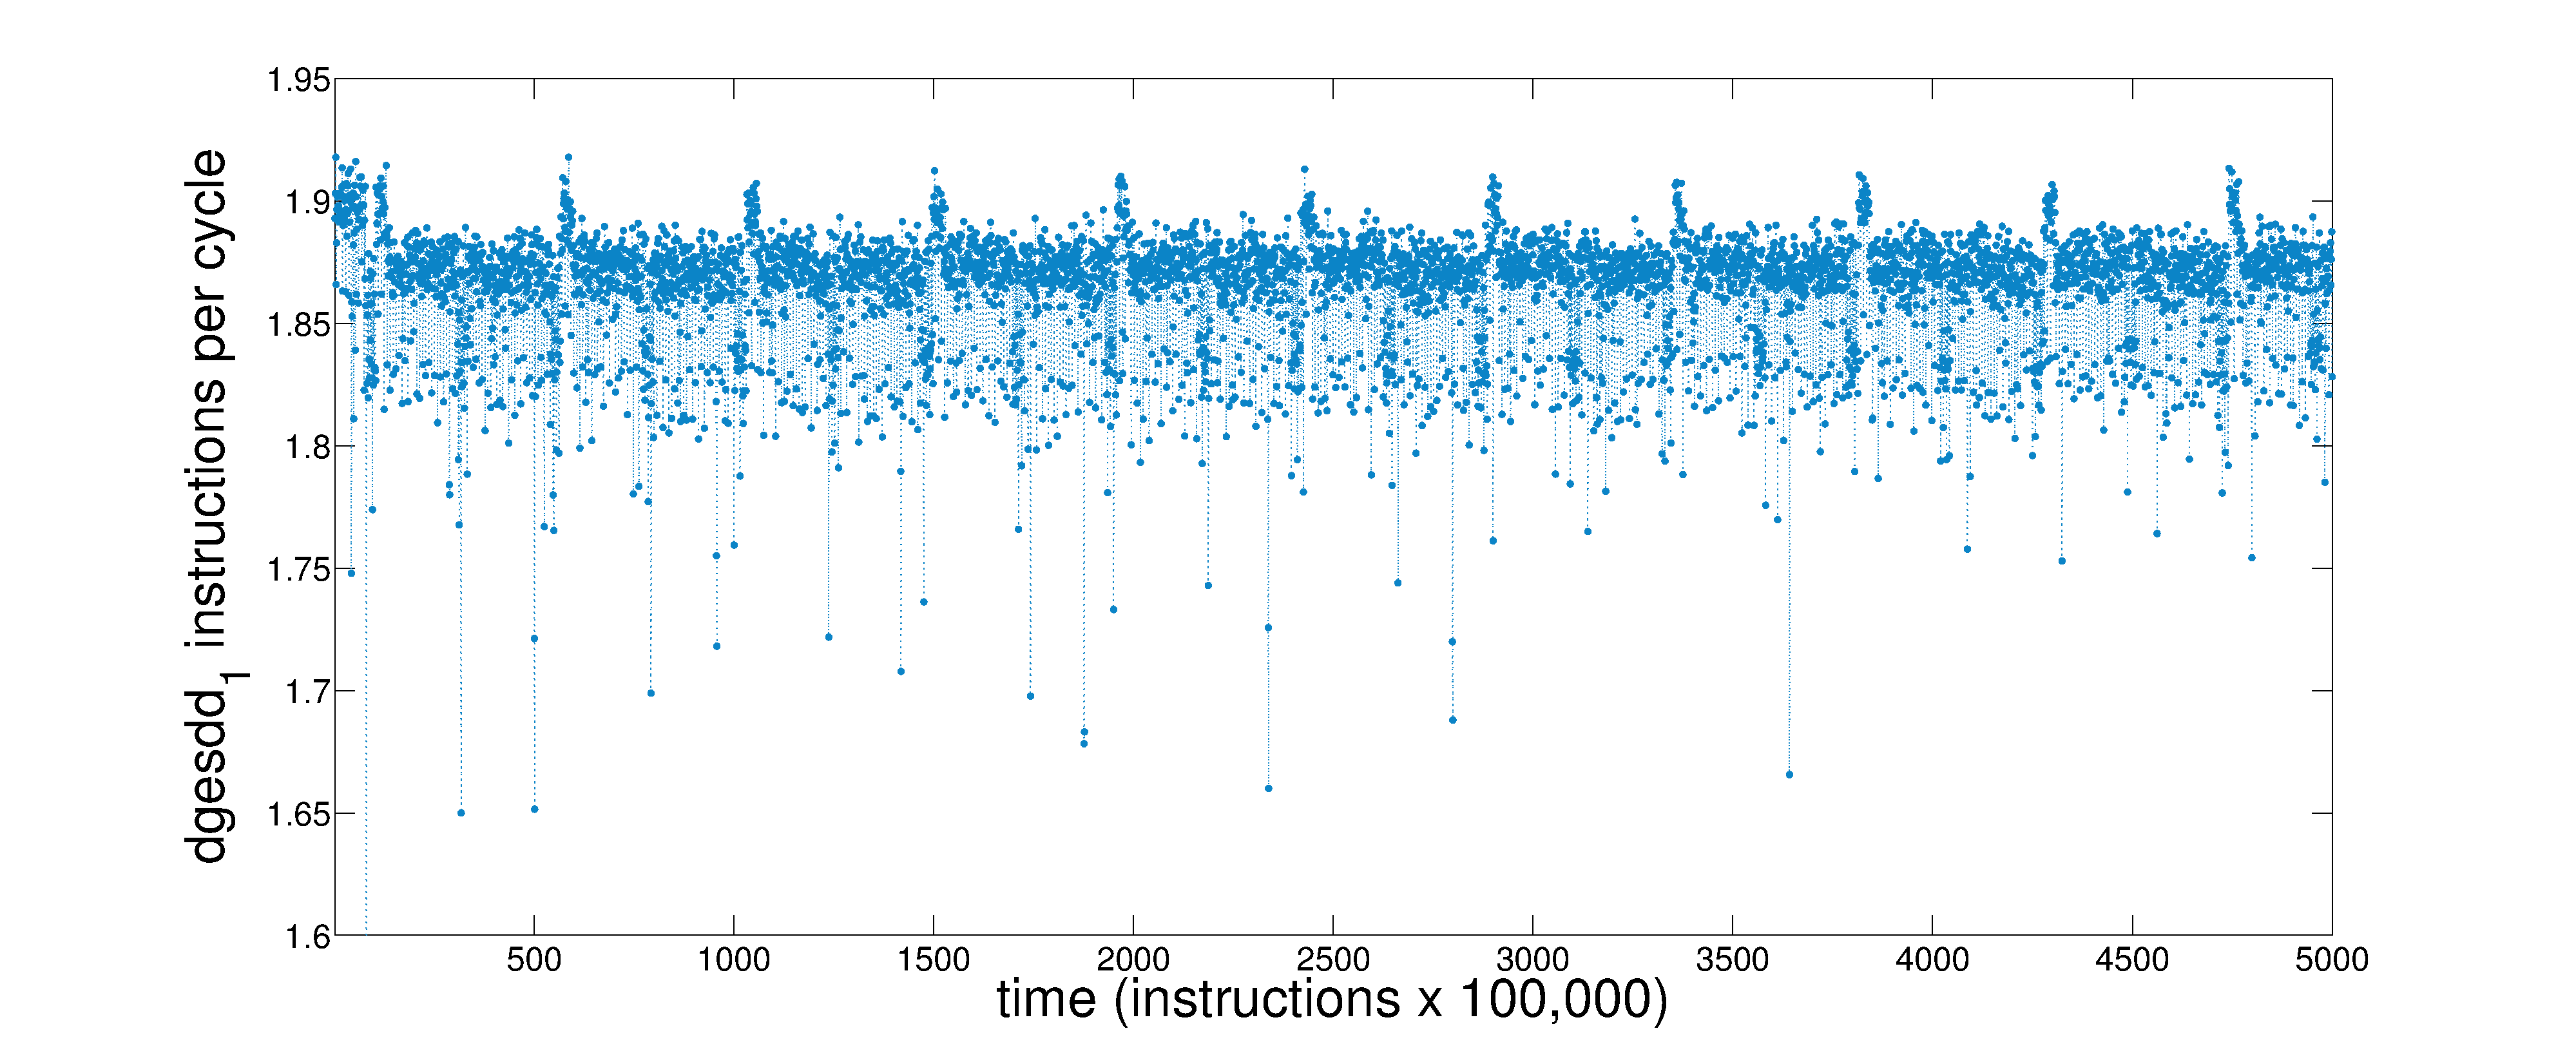
\includegraphics[width=\textwidth]{figs/svdonets2}
\caption{ For each of these, the word length used is $6$. The MASE values for LMA against ARIMA. The dashed line is the identity, delineating the traces for which either LMA or ARIMA performed better. All traces except those from \svd$_1$ lie above the line, indicating that LMA is better suited prediction method for the computer traces considered.}\label{fig:svdone-ts}  
\end{figure} 
As can be seen in Figure \ref{fig:svdone-ts}, \svdone has a highly unstructured small band on top, which is approximately 0.05 instructions per cycle wide. Approximately 80\% of the signal exists within this band of noise, this causes the WPE to be driven up as many words are being omitted by this band of the signal. The remaining 20\% of the signal are drops in instructions per cycle away from this band, ranging in size from 0.1 to 0.6 instructions per cycle\footnote{Some of the large drops are not shown for the sake of clarity of the smaller scale}. These drastic drops seem to happen every 5-7 points but the drop locations are inconsistent as well as the drops magnitude (ranging from 0.1-0.6 instructions per cycle). As discussed in Section \ref{sec:RWMethod} drops of this fashion are the bane of random walk forecasting. At every one of these drops a random walk predictor would produce two forecasts with an error 2-12 times the magnitude of the smaller band, i.e., about 40\% of the time the random walk forecast would predict with error 2-12 times the magnitude of the scale exhibited by $\approx$80\% of the signal. This inconsistency in random walk would cause cause random walk error to be high and as a result MASE scores to be artificially low. The combination of a band of noise with a high number of random drops is a weakness of this method which is present in \svdone and as a result makes this signal an outlier.


[[Joshua: I am not sure if this paragraph is strong enough or even worth having]]These results support that time series with low to moderate complexity ($0\le WPE \le 0.85$) can be predicted more efficiently than a na\"ive random walk \emph{and} that complexity can be qualitatively measured for a real-valued noisy time series using WPE. This will allow practitioners to stop spinning their wheels in the case of signals who are simply better predicted with a simple strategy like random walk. The analysis of these results illuminates an interesting point: The way structure, information and complexity are processed by a generating process plays a crucial role in the success of a given prediction scheme. 











%This portion should justify the following claim%%%%%%%%%%%%%%%%%%%%%%
%\item The way structure/information/complexity is processed internally by a given process plays a crucial role in predictability.
%%%%%%%%%%%%%%%%%%%%%%%%%






Comparing Figures~\ref{fig:lma_pred_vs_ent} and \ref{fig:arima_pred_vs_ent} also elucidates another key finding: usable and quantifiable predictive structure can be present in a time series without a prediction scheme being able to utilize it. In particular, information may be transferred from past to future through the present but because of the mechanism the underlying process uses to process that information  (e.g., linear or nonlinear) certain prediction strategies may be blind to or not be able to efficiently utilize this information. For example, consider \col, programs like this have been shown to exhibit deterministic chaos \cite{mytkowicz09}. If this were the case with \col, an out-of-the-box linear method like ARIMA would simply be ill-equipped to model and utilize the kind of structure present, as is evident in Figure \ref{fig:arima_pred_vs_ent}. In contrast, a nonlinear predictor like LMA which is built to handle deterministic chaos, can interpret and utilize this type of structure just fine. We believe that many of the shifts in forecast accuracy for low-to-moderate WPE programs between ARIMA and LMA is precisely happening for this reason: Just because there is forward information transfer, does not mean that an arbitrary predictor can interpret or utilize it, but luckily WPE can tell us when this structure is present as shown in Figure \ref{fig:lma_vs_arima}.

%In Figures~\ref{fig:lma_pred_vs_ent} and \ref{fig:arima_pred_vs_ent} we directly compare the performance of the LMA and ARIMA prediction methods (respectively) to the value of the weighted permutation entropy for all runs of each program under consideration. The LMA MASE values are largely similar to those of the best predictions, primarily because LMA often performed superior to ARIMA (and the na\"ive method). On the other hand, the ARIMA MASE values are largely uncorrelated with WPE values. As was hinted at while discussing the previous results, the fact that ARIMA is uncorrelated with WPE brings about an interesting perspective on information transfer and WPE. The WPE is sensitive to both linear and nonlinear structure. When you have a low WPE and a high ARIMA it could be that the structure WPE is picking up is simply nonlinear structure that LMA can handle but ARIMA cannot. So while ARIMA is consistently out performed by random walk,  there is plenty of structure present as suggested by WPE and taken advantage of by LMA but since it is nonlinear ARIMA can't take it into account and does bad.



%is in large part one of the major findings of this work. More specifically, say we tried to predict an arbitrary noisy real-valued time series with an ``out-of-the-box" prediction strategy like ARIMA as proposed in \cite{autoArima} and say we got inconsistent and bad forecasts, (i.e., perform worse than the na\"ive random walk strategy (MASE$>1$). How do we determine if the prediction strategy is not adequate for the prediction task, or if the signal is simply too complex to predict. If a signal is too complex and too little forward information transfer is present we may not be able to do better than the random walk, in which case we should not worry ourselves over finding a more complicated prediction strategy. However, if we measure the complexity to be low, $\textrm{WPE}<0.85$ (see Fig.~\ref{fig:pred_vs_wpe}) we can most likely do much better than the random walk and should search for more adequate prediction strategies. 




 


Other noteworthy features of the LMA and ARIMA results are the cluster locations
and distributions. The WPE values of each run of any particular program tend to
have little variance, leading to the clusters in
Figures~\ref{fig:arima_pred_vs_ent} and \ref{fig:lma_pred_vs_ent} to be fairly
constrained in the $y$ direction. For most traces, the LMA and ARIMA variance is
low as well, resulting is small, tight clusters. The ARIMA MASE values of the \col
traces, however, have a large variance resulting in the spread seen in
Figure~\ref{fig:arima_pred_vs_ent}. Not only are the MASE values of that cluster
bad, in that other predictors vastly outperform it, but they are inconsistent.
Furthermore, since LMA can predict nonlinear behavior while ARIMA cannot, we
see that the clusters in Figure ~\ref{fig:arima_pred_vs_ent} are mostly further to
the right than those in Figure~\ref{fig:lma_pred_vs_ent}.



\section{ Conclusions \& Future Work}\label{sec:conc}

[[Joshua: These need to be rewritten to conclude and address this paper...]]


The results presented here suggest that permutation entropy---a ordinal
calculation of forward information transfer in a time series---is an effective
metric for predictability of computer performance traces. Experimentally, traces
with a persistent PE $\gtrapprox 0.97$ have a natural level of complexity that
may overshadow the inherent determinism in the system dynamics, whereas traces
with PE $\lessapprox 0.7$ seem to be highly predictable (viz., at least an order
of magnitude improvement in nRMSPE).Further, the persistent WPE values of 0.5--
0.6 for the {\tt col\_major} trace are consistent with dynamical chaos, further
corroborating the results of~\cite{mytkowicz09}.

If information is the limit, then gathering and using more information is an
obvious next step.  There is an equally obvious tension here between data length
and prediction speed: a forecast that requires half a second to compute is not
useful for the purposes of real-time control of a computer system with a MHz
clock rate.  Another alternative is to sample several system variables
simultaneously and build multivariate delay-coordinate embeddings.  Existing
approaches to that are computationally prohibitive
\cite{cao-multivariate-embedding}.  We are working on alternative
methods that sidestep that complexity.

%%This use of permutaiotn entropy is a useful application of information
%%theory to computer performance modeling because it gives you a simple
%%and fast way to decide whether building a model and trying to forecast
%%the future is worthwhile or if guessing the mean is just as effective.
%%End with a sentence tying back to power management and world peace.


%\begin{it}
%Summarize the results.

%Paragraphs on the issues that come up, including one about the "amount
%of info" one: if one could sample more variables, for instance, one
%might be able to do a better job of predicting more-complex traces.
%Segue to some handwaving about multivariable LMA models; tie this back
%to the "computers are NLD systems" stuff in the intro.  This is a real
%challenge; current approaches to this modelling problem have the major
%issue of taking way too long to build.  And that's a big issue if
%you're trying not just to classify, but to predict.  In a system that
%runs at MHz speeds, a prediction that takes milliseconds to compute is
%not useful.
%\end{it}







\section*{Acknowledgment}
This work was partially supported by NSF grant \#CMMI-1245947 and ARO
grant \#W911NF-12-1-0288.

\bibliographystyle{unsrt}
\bibliography{bibliofile}


\end{document}
